 \documentclass[
  	11pt,% tamanho da fonte
 	openright,% capítulos começam em pág ímpar (insere página vazia caso preciso)
 	twoside,% para impressão em verso e anverso. Oposto a oneside
 	a4paper,% tamanho do papel. 
 	english,% idioma adicional para hifenização
 	brazil % o último idioma é o principal do documento
 	]{abntex2}
	
% \documentclass[sumario=abnt-6027-2012,12pt,twoside,a4paper,english,brazil]{abntex2} % do cabelo

% ---
% Cabelo sugeriu a fonte georgia
% ---
% \usepackage{pslatex}
\usepackage[table,xcdraw]{xcolor}
\usepackage{lmodern}			% Usa a fonte Latin Modern			
\usepackage[T1]{fontenc}		% Selecao de codigos de fonte.
\usepackage[utf8]{inputenc}		% Codificacao do documento (conversão automática dos acentos)
\usepackage{lastpage}			% Usado pela Ficha catalográfica
\usepackage{indentfirst}		% Indenta o primeiro parágrafo de cada seção.
\usepackage{color}				% Controle das cores
\usepackage{graphicx}			% Inclusão de gráficos
\usepackage{microtype} 			% para melhorias de justificação
% \usepackage[brazilian,hyperpageref]{backref}	 % Paginas com as citações na bibl
\usepackage[num]{abntex2cite}	% Citações padrão ABNT
% \usepackage[square]{abntex2cite}	% Citações padrão ABNT
\citebrackets[] 

\renewcommand{\familydefault}{\rmdefault}

\renewcommand{\ABNTEXchapterfont}{\fontfamily{\rmdefault}\fontseries{b}\selectfont}
\renewcommand{\ABNTEXsectionfont}{\fontfamily{\rmdefault}\fontseries{b}\selectfont}
\renewcommand{\ABNTEXsubsectionfont}{\fontfamily{\rmdefault}\fontseries{b}\selectfont}
\renewcommand{\ABNTEXsubsubsectionfont}{\fontfamily{\rmdefault}\fontseries{b}\selectfont}
\renewcommand{\ABNTEXchapterfontsize}{\fontsize{14pt}{17pt}}
\renewcommand{\ABNTEXsectionfontsize}{\fontsize{12pt}{15pt}}
\renewcommand{\ABNTEXsubsectionfontsize}{\fontsize{12pt}{15pt}}
\renewcommand{\ABNTEXsubsubsectionfontsize}{\fontsize{12pt}{15pt}}
 
% --- 
% CONFIGURAÇÕES DE PACOTES
% --- 

%   % ---
%   % Configurações do pacote backref
%   % Usado sem a opção hyperpageref de backref
%   \renewcommand{\backrefpagesname}{Citado na(s) página(s):~}
%   % Texto padrão antes do número das páginas
%   \renewcommand{\backref}{}
%   % Define os textos da citação
%   \renewcommand*{\backrefalt}[4]{
% 	  \ifcase #1 %
% 		  Nenhuma citação no texto.%
% 	  \or
% 		  Citado na página #2.%     OI JOAO ESSA PARTE AQUI DE `CITADO X VEZES` NAO E NECESSARIA BJS
% 	  \else
% 		  Citado #1 vezes nas páginas #2.%
% 	  \fi}%
%   % ---

% ---
% Informações de dados para CAPA e FOLHA DE ROSTO
% ---
\titulo{Implementação de uma plataforma de teste de estratégia de controle de VANTs utilizando robô terrestre autônomo de alta velocidade}
\autor{João Victor Batista Gordo}
\local{São Carlos, Brasil}
\data{\today}
\orientador{Eduardo do Valle Simões}
\instituicao{
  Universidade de São Paulo
  \par
Escola de Engenharia de São Carlos
  \par
Departamento de Engenharia Elétrica e de Computação}
\tipotrabalho{Monografia do Trabalho de Conclusão de Curso}
% O preambulo deve conter o tipo do trabalho, o objetivo, 
% o nome da instituição e a área de concentração 
\preambulo{} % TODO fazer isso direitinho
% ---


% ---
% Configurações de aparência do PDF final

% alterando o aspecto da cor azul
\definecolor{blue}{RGB}{41,5,195}

% informações do PDF
\makeatletter
\hypersetup{
     	%pagebackref=true,
		pdftitle={\@title}, 
		pdfauthor={\@author},
    	pdfsubject={\imprimirpreambulo},
	    pdfcreator={LaTeX with abnTeX2},
		pdfkeywords={navegação autônoma}{robótica}{sistemas reativos}{desvio de obstáculos}{...?}, % TODO
		colorlinks=true,       		% false: boxed links; true: colored links
    	linkcolor=blue,          	% color of internal links
    	citecolor=blue,        		% color of links to bibliography
    	filecolor=magenta,      		% color of file links
		urlcolor=blue,
		bookmarksdepth=4
}
\makeatother

% --- 
% Espaçamentos entre linhas e parágrafos 
% --- 

% O tamanho do parágrafo é dado por:
\setlength{\parindent}{1.3cm}

% Controle do espaçamento entre um parágrafo e outro:
\setlength{\parskip}{0.2cm}  % tente também \onelineskip

% ---
% compila o indice
% ---
\makeindex
% ---

% ----
% Início do documento
% ----
\begin{document}

% Retira espaço extra obsoleto entre as frases.
\frenchspacing 
% ----------------------------------------------------------
% ELEMENTOS PRÉ-TEXTUAIS
% ----------------------------------------------------------
% \pretextual

% ---
% Capa
% ---
\imprimircapa
% ---

% ---
% Folha de rosto
% (o * indica que haverá a ficha bibliográfica)
% ---
\imprimirfolhaderosto*
% ---

% ---
% Inserir a ficha bibliografica     OBS.: tirei o código que tinha aqui!
% ---
% \includepdf{fichabibliografica_final.pdf}

% ---
% Inserir folha de aprovação
% ---
%
% \includepdf{folhadeaprovacao_final.pdf}
%

% ---
% Dedicatória
% ---
\begin{dedicatoria}
   \vspace*{\fill}
   \centering
   \noindent
   \textit{ Este trabalho é dedicado às crianças adultas que,\\
   quando pequenas, sonharam em se tornar cientistas.} \vspace*{\fill}
\end{dedicatoria}
% ---

% ---
% Agradecimentos
% ---
\begin{agradecimentos}
Eu gostaria de agradecer à comunidade que vive o paradigma revolucionário de disseminação livre e gratuita de ideias e trabalhos.
Este projeto é um fruto tímido de uma árvore regada pelos esforços de cada uma destas pessoas que, de gota em gota, clareiam as águas 
turvadas pelo egoísmo e nutrem a germinação de verdadeiros pomares que estão por vir. Quem sabe um dia o único obstáculo ao aprendizado e construção 
do conhecimento seja a força de vontade...
\end{agradecimentos}
% ---

% ---
% Epígrafe
% ---
\begin{epigrafe}
    \vspace*{\fill}
	\begin{flushright}
		\textit{``Não vos amoldeis às estruturas deste mundo, \\
		mas transformai-vos pela renovação da mente, \\
		a fim de distinguir qual é a vontade de Deus: \\
		o que é bom, o que Lhe é agradável, o que é perfeito.\\
		(Bíblia Sagrada, Romanos 12, 2)}
	\end{flushright}
\end{epigrafe}
% ---

% ---
% RESUMOS
% ---

% resumo em português
\setlength{\absparsep}{18pt} % ajusta o espaçamento dos parágrafos do resumo
\begin{resumo}
%  Segundo a \citeonline[3.1-3.2]{NBR6028:2003}, o resumo deve ressaltar o
 objetivo, o método, os resultados e as conclusões do documento. A ordem e a extensão
 destes itens dependem do tipo de resumo (informativo ou indicativo) e do
 tratamento que cada item recebe no documento original. O resumo deve ser
 precedido da referência do documento, com exceção do resumo inserido no
 próprio documento. (\ldots) As palavras-chave devem figurar logo abaixo do
 resumo, antecedidas da expressão Palavras-chave:, separadas entre si por
 ponto e finalizadas também por ponto.

 \textbf{Palavras-chaves}: latex. abntex. editoração de texto.
\end{resumo}

% resumo em inglês
\begin{resumo}[Abstract]
 \begin{otherlanguage*}{english}
   This is the english abstract.

   \vspace{\onelineskip}
 
   \noindent 
   \textbf{Key-words}: latex. abntex. text editoration.
 \end{otherlanguage*}
\end{resumo}


% ---
% inserir lista de ilustrações
% ---
\pdfbookmark[0]{\listfigurename}{lof}
\listoffigures*
\cleardoublepage
% ---

% ---
% inserir lista de tabelas
% ---
\pdfbookmark[0]{\listtablename}{lot}
\listoftables*
\cleardoublepage
% ---

% ---
% inserir lista de abreviaturas e siglas
% ---
\begin{siglas}
  \item[CC] Corrente Contínua
  \item[PWM] \textit{Pulse Width Modulation}
  \item[ESC] \textit{Electronic Speed Controller}
  \item[IDE] \textit{Integrated Development Environment}
  \item[ISM] \textit{Industrial, Scientific and Medical}
  \item[UHF] \textit{Ultra High Frequency}
  \item[SPI] \textit{Serial Peripheral Interface} 
  \item[USB] \textit{Universal Serial Bus}
  \item[CRC] \textit{Cyclic Redundancy Check}
  \item[GFSK] \textit{Gaussian Frequency Shift Keying}
  \item[BLDC] \textit{Brushless Direct Current}
  \item[FIFO] \textit{First In First Out}
  \item[VANT] \textit{Veículo Aereo Não Tripulado}
  \item[UBEC] \textit{Ultimate Batterie Eliminator Circuit}
  \item[LiPo] Lítio Polímero
  \item[MIFA] \textit{Meandered Inverted-F Antenna}
  \item[ICSP] \textit{In-Circuit Serial Programming}
\end{siglas}
% ---

% ---
% inserir lista de símbolos
% ---
\begin{simbolos}
  \item[$ \alpha $] coeficiente de atenuação do meio.
  \item[$ \tau $] tempo de meia volta da onda propagante, i.e. \textit{time of flight}, do sensor.
  \item[$ \Delta $] distância medida nos sensores do tipo \textit{time of flight}.
  \item[$ \nu $] velocidade de propagação no meio da onda ou partícula nos sensores do tipo \textit{time of flight}.
%   \item[$\approx$] aproximadamente.
\end{simbolos}
% ---

% ---
% inserir o sumario
% ---
\pdfbookmark[0]{\contentsname}{toc}
\tableofcontents*
\cleardoublepage
% ---



% ----------------------------------------------------------
% ELEMENTOS TEXTUAIS
% ----------------------------------------------------------
\textual

 \chapter{Introdução}
O presente trabalho consiste na implementação de um veículo autônomo de alta
velocidade, desenvolvido sob o paradigma de sistemas puramente reativos, cuja finalidade
é servir como uma plataforma terrestre de testes de estratégias de navegação de Veículos
Aereos Não Tripulados, VANTs, dentro da arquitetura MOSA, \textit{Mission Oriented Sensor
Array}. Isto é, na arquitetura MOSA, o escopo deste projeto consiste na porção relativa
ao controlador de navegação, que é responsável por cuidar da integridade da aeronave, enquanto a parte
orientada à missão é o que pretende-se testar utilizando o veículo. A necessidade de
se desenvolver um veículo terrestre para testar estratégias de voo se dá pelo fato de que este é
um sistema embarcado crítico cuja falha pode resultar em acidentes graves, logo, caso o
comportamento do MOSA desenvolvido seja extensivamente testado em um ambiente livre
de riscos utilizando-se o veículo, há menos risco de eventuais danos provocados por mal
funcionamento. 
Como o intuito do projeto é simular um \textit{drone} para testar novos algoritmos de navegação para que 
se tenha uma segurança maior no funcionamento desejado do \textit{software} antes de serem feitos os devidos 
testes utilizando de fato uma aeronave, o veículo desenvido opera em velocidades similares às de VANTs,
podendo atingir até \unitfrac[100]{km}{h}.
Maiores detalhes acerca da arquitetura MOSA serão abordados na seção
de Embasamento Teórico.

O projeto pode ser dividido em 4 subsistemas: percepção, locomoção, comunicação
e navegação. A percepção é feita através de uma matriz de cinco sensores ultrassônicos
de baixo custo, que são disparados simultaneamente a fim de reduzir o tempo gasto
com obtenção dos dados do ambiente externo. Como consequência disso, obtém-se dados
menos confiáveis pois são intensificados efeitos colaterais como o crosstalk, que não pode ser
eliminado processando medidas consecutivas, conforme \citeonline{2016_artigo_1}. Além disso, buscou-se verificar
o quão significativo é o impacto na confiabilidade das medidas caso os ciclos de leitura dos
sonares seja determinado de acordo com as circunstâncias do meio, isto é, caso não haja
um intervalo de medição fixo e pré-determinado, denominado intervalo estático de agora
em diante, de modo que o período gasto na percepção estivesse atrelado apenas ao tempo
gasto pelo sonar que detectou o obstáculo mais distante do veículo, denominado intervalo
dinâmico. Ao adotar intervalos dinâmicos, reduz-se o tempo entre leituras consecutivas,
o que pode fazer com que vibrações residuais da membrana responsável por emitir as
ondas acústicas sensibilize o elemento receptor provocando falsas leituras, conforme \citeonline{jones}.
Maiores detalhes acerca do princípio de funcionamento dos sensores ultrassônicos, assim
como vantagens e desvantagens deste sensor encontram-se na seção de Materiais desta
monografia.

Para a locomoção do veículo, são utilizados dois motores \textit{brushless} de corrente
contínua, de modo que a tração é dianteira. Logo, o veículo faz curvas em razão da diferença
de velocidade entre os BLDC e, por se tratar de motores usualmente utilizados em VANTs,
atinge velocidade de até  \unitfrac[80]{km}{h}.
Como o controle de motores sem escovas não é trivial de
ser feito, foram utilizados controladores eletrônicos de velocidade, ESCs, como elemento
intermediador entre o microcontrolador e os motores. Desta forma, todo o tratamento de
mais baixo nível no que concerne o acionamento das bobinas dos motores foi designado
a este dispositivo, enquanto o microcontrolador se responsabiliza por fornecer aos ESCs
a velocidade que pretende-se obter do seu respectivo motor.
O sistema de comunicação tem o propósito de: fornecer feedback dos dados internos
do veículo, como percepção e velocidade dos motores; regular o acionamento dos motores,
pois repassa ao microcontrolador informações de um botão de segurança, que emite sinais
ao veículo, autorizando-o ou não a navegar; e, finalmente, de servir como uma interface de
comandos na qual é possível controlar remotamente o veículo.
\footnote{Entenda-se por veículo não só a parte física como rodas, motores e dispositivos mas, também, todo o \textit{software} responsável por gerir 
o automóvel.}.

Quanto ao subsistema de navegação, temos que este consiste na inteligência artificial
do veículo, isto é, qual é a estratégia utilizada para efetuar o desvio de obstáculos com
base nos dados colhidos pelos sonares. A técnica de desvio de obstáculos implementada
é a mais simples possível: trata-se de uma função que mapeia as leituras dos sonares -
categorizadas em três regiões: perigo, atenção e distante - em um par de velocidades
angulares - categorizados quanto a intensidade em forte, médio e leve, e quanto à direção
em esquerda ou direita - a serem impostas aos motores de acordo com qual a combinação
de regiões lida pela matriz de sonares, conforme a Eq. \ref{nav}. A tabela verdade que relaciona
domínio e contradomínio da função de desvio de obstáculos consta no Apêndice, vide Tabela \ref{IA}.

\begin{equation}
\label{nav}
T:R^5 \rightarrow S
\end{equation}
$$\quad \textrm{em que:} \quad R=\{distante, perigo, atenção\}, \quad S=\{E_L, E_M, E_F, D_L, D_M, D_F\}$$

Note que cada um dos elementos do conjunto S são pares ordenados que representam a
velocidade angular dos motores.

\begin{table}[!htb]
\centering
\caption{}
\label{IA}
\begin{tabular}{|ccccc|c|}
\hline
{\color[HTML]{00009B} \textbf{$USS_0$}} & {\color[HTML]{00009B} \textbf{$USS_1$}} & {\color[HTML]{00009B} \textbf{$USS_2$}} & 
{\color[HTML]{00009B} \textbf{$USS_3$}} & {\color[HTML]{00009B} \textbf{$USS_4$}} & {\color[HTML]{FE0000} \textbf{Ação}} \\ 
\hline
{\color[HTML]{00009B} 0}                                     & {\color[HTML]{00009B} 0}                                    & {\color[HTML]{00009B} 0} 
 
                                  & {\color[HTML]{00009B} 0}                                    & {\color[HTML]{00009B} 1}                            
 
       & {\color[HTML]{FE0000} $E_L$}                                     \\ \hline
{\color[HTML]{00009B} 0}                                     & {\color[HTML]{00009B} 0}                                    & {\color[HTML]{00009B} 0} 
 
                                  & {\color[HTML]{00009B} 1}                                    & {\color[HTML]{00009B} 0}                            
 
       & {\color[HTML]{FE0000} $E_M$}                                     \\ \hline
{\color[HTML]{00009B} 0}                                     & {\color[HTML]{00009B} 0}                                    & {\color[HTML]{00009B} 0} 
 
                                  & {\color[HTML]{00009B} 1}                                    & {\color[HTML]{00009B} 1}                            
 
       & {\color[HTML]{FE0000} $E_M$}                                     \\ \hline
{\color[HTML]{00009B} 0}                                     & {\color[HTML]{00009B} 0}                                    & {\color[HTML]{00009B} 1} 
 
                                  & {\color[HTML]{00009B} 0}                                    & {\color[HTML]{00009B} 0}                            
 
       & {\color[HTML]{FE0000} $E_F$}                                     \\ \hline
{\color[HTML]{00009B} 0}                                     & {\color[HTML]{00009B} 0}                                    & {\color[HTML]{00009B} 1} 
 
                                  & {\color[HTML]{00009B} 0}                                    & {\color[HTML]{00009B} 1}                            
 
       & {\color[HTML]{FE0000} $E_F$}                                     \\ \hline
{\color[HTML]{00009B} 0}                                   & {\color[HTML]{00009B} 0}                                    & {\color[HTML]{00009B} 1}   
 
                                & {\color[HTML]{00009B} 1}                                    & {\color[HTML]{00009B} 0}                              
 
     & {\color[HTML]{FE0000} $E_F$}                                     \\ \hline
{\color[HTML]{00009B} 0}                                    & {\color[HTML]{00009B} 0}                                  & {\color[HTML]{00009B} 1}    
 
                               & {\color[HTML]{00009B} 1}                                    & {\color[HTML]{00009B} 1}                               
 
    & {\color[HTML]{FE0000} $E_F$}                                     \\ \hline
{\color[HTML]{00009B} 0}                                     & {\color[HTML]{00009B} 1}                                    & {\color[HTML]{00009B} 0} 
 
                                & {\color[HTML]{00009B} 0}                                    & {\color[HTML]{00009B} 0}                              
 
     & {\color[HTML]{FE0000} $D_M$}                                     \\ \hline
{\color[HTML]{00009B} 0}                                    & {\color[HTML]{00009B} 1}                                    & {\color[HTML]{00009B} 0}  
 
                                 & {\color[HTML]{00009B} 0}                                 & {\color[HTML]{00009B} 1}                                
 
   & {\color[HTML]{FE0000} $D_M$}                                     \\ \hline
{\color[HTML]{00009B} 0}                                    & {\color[HTML]{00009B} 1}                                    & {\color[HTML]{00009B} 0}  
 
                                 & {\color[HTML]{00009B} 1}                                    & {\color[HTML]{00009B} 0}                             
 
      & {\color[HTML]{FE0000} $E_F$}                                     \\ \hline
{\color[HTML]{00009B} 0}                                    & {\color[HTML]{00009B} 1}                                    & {\color[HTML]{00009B} 0}  
 
                                 & {\color[HTML]{00009B} 1}                                    & {\color[HTML]{00009B} 1}                             
 
      & {\color[HTML]{FE0000} $E_M$}                                  \\ \hline
{\color[HTML]{00009B} 0}                                     & {\color[HTML]{00009B} 1}                                    & {\color[HTML]{00009B} 1} 
 
                                  & {\color[HTML]{00009B} 0}                                    & {\color[HTML]{00009B} 0}                            
 
       & {\color[HTML]{FE0000} $D_F$}                                     \\ \hline
{\color[HTML]{00009B} 0}                                     & {\color[HTML]{00009B} 1}                                    & {\color[HTML]{00009B} 1} 
 
                                  & {\color[HTML]{00009B} 0}                                    & {\color[HTML]{00009B} 1}                            
 
       & {\color[HTML]{FE0000} $E_F$}                                     \\ \hline
{\color[HTML]{00009B} 0}                                     & {\color[HTML]{00009B} 1}                                    & {\color[HTML]{00009B} 1} 
 
                                  & {\color[HTML]{00009B} 1}                                    & {\color[HTML]{00009B} 0}                            
 
       & {\color[HTML]{FE0000} $E_F$}                                     \\ \hline
{\color[HTML]{00009B} 0}                                     & {\color[HTML]{00009B} 1}                                    & {\color[HTML]{00009B} 1} 
 
                                  & {\color[HTML]{00009B} 1}                                    & {\color[HTML]{00009B} 1}                            
 
       & {\color[HTML]{FE0000} $E_F$}                                     \\ \hline
{\color[HTML]{00009B} 1}                                     & {\color[HTML]{00009B} 0}                                    & {\color[HTML]{00009B} 0} 
 
                                  & {\color[HTML]{00009B} 0}                                    & {\color[HTML]{00009B} 0}                            
 
       & {\color[HTML]{FE0000} $D_L$}                                     \\ \hline
{\color[HTML]{00009B} 1}                                     & {\color[HTML]{00009B} 0}                                    & {\color[HTML]{00009B} 0} 
 
                                  & {\color[HTML]{00009B} 0}                                    & {\color[HTML]{00009B} 1}                            
 
       & {\color[HTML]{FE0000} Frente}                                     \\ \hline
{\color[HTML]{00009B} 1}                                     & {\color[HTML]{00009B} 0}                                    & {\color[HTML]{00009B} 0} 
 
                                  & {\color[HTML]{00009B} 1}                                    & {\color[HTML]{00009B} 0}                            
 
       & {\color[HTML]{FE0000} $E_M$}                                     \\ \hline
{\color[HTML]{00009B} 1}                                     & {\color[HTML]{00009B} 0}                                    & {\color[HTML]{00009B} 0} 
 
                                  & {\color[HTML]{00009B} 1}                                    & {\color[HTML]{00009B} 1}                            
 
       & {\color[HTML]{FE0000} $E_M$}                                     \\ \hline
{\color[HTML]{00009B} 1}                                     & {\color[HTML]{00009B} 0}                                    & {\color[HTML]{00009B} 1} 
 
                                  & {\color[HTML]{00009B} 0}                                    & {\color[HTML]{00009B} 0}                            
 
       & {\color[HTML]{FE0000} $D_F$}                                     \\ \hline
{\color[HTML]{00009B} 1}                                     & {\color[HTML]{00009B} 0}                                    & {\color[HTML]{00009B} 1} 
 
                                  & {\color[HTML]{00009B} 0}                                    & {\color[HTML]{00009B} 1}                            
 
       & {\color[HTML]{FE0000} $E_F$}                                     \\ \hline
{\color[HTML]{00009B} 1}                                     & {\color[HTML]{00009B} 0}                                    & {\color[HTML]{00009B} 1} 
 
                                  & {\color[HTML]{00009B} 1}                                    & {\color[HTML]{00009B} 0}                            
 
       & {\color[HTML]{FE0000} $E_F$}                                     \\ \hline
{\color[HTML]{00009B} 1}                                     & {\color[HTML]{00009B} 0}                                    & {\color[HTML]{00009B} 1} 
 
                                  & {\color[HTML]{00009B} 1}                                    & {\color[HTML]{00009B} 1}                            
 
       & {\color[HTML]{FE0000} $E_F$}                                     \\ \hline
{\color[HTML]{00009B} 1}                                     & {\color[HTML]{00009B} 1}                                    & {\color[HTML]{00009B} 0} 
 
                                  & {\color[HTML]{00009B} 0}                                    & {\color[HTML]{00009B} 0}                            
 
       & {\color[HTML]{FE0000} $D_M$}                                     \\ \hline
{\color[HTML]{00009B} 1}                                     & {\color[HTML]{00009B} 1}                                    & {\color[HTML]{00009B} 0} 
 
                                  & {\color[HTML]{00009B} 0}                                    & {\color[HTML]{00009B} 1}                            
 
       & {\color[HTML]{FE0000} $D_M$}                                     \\ \hline
{\color[HTML]{00009B} 1}                                     & {\color[HTML]{00009B} 1}                                    & {\color[HTML]{00009B} 0} 
 
                                  & {\color[HTML]{00009B} 1}                                    & {\color[HTML]{00009B} 0}                            
 
       & {\color[HTML]{FE0000} $D_M$}                                     \\ \hline
{\color[HTML]{00009B} 1}                                     & {\color[HTML]{00009B} 1}                                    & {\color[HTML]{00009B} 0} 
 
                                  & {\color[HTML]{00009B} 1}                                    & {\color[HTML]{00009B} 1}                            
 
       & {\color[HTML]{FE0000} Frente}                                     \\ \hline
{\color[HTML]{00009B} 1}                                     & {\color[HTML]{00009B} 1}                                    & {\color[HTML]{00009B} 1} 
 
                                  & {\color[HTML]{00009B} 0}                                    & {\color[HTML]{00009B} 0}                            
 
       & {\color[HTML]{FE0000} $D_F$}                                     \\ \hline
{\color[HTML]{00009B} 1}                                     & {\color[HTML]{00009B} 1}                                    & {\color[HTML]{00009B} 1} 
 
                                  & {\color[HTML]{00009B} 0}                                    & {\color[HTML]{00009B} 1}                            
 
       & {\color[HTML]{FE0000} $D_F$}                                     \\ \hline
{\color[HTML]{00009B} 1}                                     & {\color[HTML]{00009B} 1}                                    & {\color[HTML]{00009B} 1} 
 
                                  & {\color[HTML]{00009B} 1}                                    & {\color[HTML]{00009B} 0}                            
 
       & {\color[HTML]{FE0000} $D_F$}                                     \\ \hline
{\color[HTML]{00009B} 1}                                     & {\color[HTML]{00009B} 1}                                    & {\color[HTML]{00009B} 1} 
 
                                  & {\color[HTML]{00009B} 1}                                    & {\color[HTML]{00009B} 1}                            
 
       & {\color[HTML]{FE0000} $E_F$}                                    \\ \hline

\end{tabular}
\end{table}



A título de ilustração, para deixar mais claro o propósito deste projeto, podemos
supor que um MOSA esteja sendo desenvolvido com o propósito de percorrer uma rota
previamente selecionada, utilizando-se de GPS, acelerômetro e magnetômetro para a
missão. Este poderia ser testado no veículo antes de ser colocado para voar, de forma que
o veículo autônomo desempenharia a função da aeronave, sendo responsável por desviar
de eventuais obstáculos quando necessário, e quando o caminho estiver livre, o controle
do veículo seria repassado ao MOSA, mas ainda sob sua supervisão. Dessa forma, quando
em posse do veículo, o MOSA desempenharia sua missão, que no exemplo citado seria
percorrer \textit{checkpoints}.
\chapter{Embasamento Teórico}
\section{Sistemas Reativos}
\epigraph{ 
	  \textit{``Representações explícitas e modelos atrapalham. No fim das contas, a melhor representação do mundo é ele mesmo.''} 
	 }
	  { Brooks, R.A \cite{brooks} - tradução livre -} 
	  
%   \begin{flushright}
% 	  \textit{``Representações explícitas e modelos atrapalham.\\
% 	  No fim das contas, a melhor representação \\
% 	  do mundo é ele mesmo.", Brooks, R.A. 
% 	  \cite{brooks} \footnote{tradução livre}}
%   \end{flushright}

\subsection{Paradigma Reativo como Robótica Bioinspirada} 

De acordo com Rodney Brooks \cite{brooks}, para o desenvolvimento da inteligência no seu sentido mais estrito e genuíno, são condições 
suficientes que o indivíduo, que denominaremos agente, tenha as seguintes faculdades: mobilidade dentro de um ambiente dinâmico no qual esteja 
inserido, percepção do que se passa nas suas adjacências e, por fim, manutenção da própria sobrevivência.
Em suma, habilidades como o raciocinar, comunicar-se, gerar conhecimento nada mais são do que comportamentos complexos, consequências simples do fato 
de existirmos e termos o poder de reagir dentro do meio em que vivemos.

Para aprofundarmos a discussão e esclarecermos como se daria esse processo de aprimoramento dos agentes, é preciso fornecer uma  definição 
mais rigorosa do termo ``comportamento''.
Numa tradução livre: ``comportamentos são mapeamentos diretos de informações sensoriais recebidas em  
padrões de ações motoras, desempenhadas para se cumprir uma tarefa. Matematicamente, seria uma função transferência que transforma dados dos 
sensores em comandos para os atuadores'' \cite{murphy}.

Nos animais, a transformação de percepção em ação está subordinada à existência de estímulos específicos, de natureza interna ou externa 
ao agente, que podem ser entendidos como sinais de controle que que permitem ou inibem determinados comportamentos \cite{murphy}.
A título de ilustração: ao avistar uma presa - informação sensorial - o predador somente a ataca - comportamento - caso esteja com fome - estímulo 
interno; ou quando afastamos a mão - comportamento - ao tocarmos uma panela quente - a informação sensorial seria a temperatura da panela enquanto o 
estímulo externo é o fato de que ela excede uma dada temperatura.

Com base em estudos da etologia, o comportamentos dos animais podem ser inatos ou aprendidos, e a sua inteligência pode ser decomposta verticalmente 
em camadas de comportamentos, cada qual acessa os sensores e atuadores do agente de maneira independente das demais \cite{murphy}.
Isto é, o indivíduo inicia sua existência com um conjunto comportamentos inatos de autopreservação mas, ao longo da sua vida, outros 
novos vão surgindo, podendo: refinar comportamentos pré-existentes, negá-los (completamente) ou agregar-se a eles sem produzir conflitos, 
i.e. trabalhando paralelamente com os que lhe são ancestrais.
Desta forma, os dois primeiros casos podem ser entendidos como uma reutilização de camadas inferiores da inteligência, enquanto o 
último consiste na adição de mais uma camada.

\subsection{Características}
Por estar embasado em ideias da etologia discutidas na seção anterior, o paradigma reativo simplesmente desconsidera a etapa de planejamento 
existente na tríade 'percepção, planejamento, ação', que sumariza o ciclo de tarefas realizadas por um sistema sob o paradigma hierárquico 
\cite{murphy,roseli}.
Em suma, os comportamentos se dão de acordo com o que o agente percebe que está acontecendo no seu entorno, não são feitas modelagens ou 
representações do ambiente externo, apenas medições locais e orientadas a comportamentos.

Em decorrência da exclusão da etapa de planejamento, robôs desenvolvidos sob o paradigma reativo costumam ser simples e apresentarem 
respostas rápidas \cite{roseli}.
Com boas práticas de projeto é possível construir uma robô com: alta coesão, pois comportamentos podem ter acesso direto aos sensores de que 
necessitam para tomar suas decisões, o que possibilita um alto grau de independência em relação a operações e dados externos entre diferentes módulos 
ou subsistemas do robô; e baixo acoplamento, pois comportamentos são independentes entre si e, portanto, há pouca ou nenhuma dependência de ligações 
e 
interfaces externas a um dado módulo \cite{murphy}.

% TODO: \subsection{Arquitetura de Subsumpção}

\section{Arquitetura MOSA}

Arquitetura que propõe dividir o sistema aéreos de navegação autônoma em dois módulos: aeronave e MOSA \cite{mosa_proposal}.

O primeiro constitui a porção crítica do sistema embarcado, i.e. segmento cuja falha pode resultar em ao menos um dos seguintes desastres: morte 
ou lesão de pessoas; destruição ou danos a propriedades, patrimônios ou equipamentos; danos ambientais \cite{safety}.
Veículos Aéreos Não Tripulados, VANTs, apresentam a tolerância de um erro grave a cada $10^5$ ou $10^9$ horas de voo \cite{hard}, o que as 
caracteriza 
como sistemas computacionais de tempo real do tipo \textit{hard}. 
Maiores esclarecimentos acerca destes jargões podem ser encontrados no apêndice.

O segundo corresponde à parte não crítica à segurança, encarregada do controle da navegação e, por conseguinte, da determinação da maior parte dos 
parâmetros de voo. É caracterizado como um conjunto de sensores inteligentes capazes de cumprir uma missão específica, ou seja, 
existe uma relação biunívoca entre missão e MOSA, dado que ele consiste no melhor arranjo de sensores para o cenário em questão. Neste contexto, a 
aeronave é vista unicamente como o meio de transporte dos sensores, enquanto que o módulo MOSA constituiria o \textquoteleft cérebro\textquoteright{}  
da plataforma, responsável pelo cumprimento da missão e por guiar a aeronave até a sua realização.

%  \begin{figure}[h]
%   \includegraphics[scale=0.5]{./Resources/MOSA.png}
%   \caption{MOSA} \label{MOSA}
%  \end{figure}

No entanto, como a aeronave é o elemento responsável pela garantia da segurança, cabe a ela acatar ou não os comandos do MOSA. E pode, inclusive, 
optar por readaptar a missão em tempo de voo para se ajustar ao cenário, o que inclui a seleção dos sensores que melhor se encaixam na dada 
conjuntura.

Isso se dá através de uma matriz de reconfiguração dinamicamente adaptável denominada \textit{Knowledge Based Framework}, seu papel é comparável à 
expertise de um piloto.
Ou seja, um elemento inteligente capaz de escolher o melhor serviço  a ser executado com base em regras e critérios de seleção como resposta em tempo 
real, segurança, performance.


% diferentes missões, definidas pelo mosa e diferentes sensores, podem ser integrados, possibilitando a escolha do melhor arranjo de sensores que se 
% ajuste ao cenário de utilização do sistema. este é o mecanismo básico do mosa, fazendo com que a missão possa ser adaptativa. durante uma missão, 
% com 
% base em uma matriz de reconfiguração o vant pode se adaptar dinamicamente às características da missão, escolhendo os sensores que melhor se 
% encaixam 
% dependendo da situação. além do hardware, um sistema mosa deve contemplar também o software capaz de realizar uma missão, comunicar-se com todos os 
% sensores que o compõe, enviar e receber dados para a aeronave .
% 
% o sistema mosa deve ser capaz de determinar se a missão prevista pode ou não ser realizada.
% 
% the aircraft can, for safety reasons, not follow the flight sensors
% commands, eventually terminating the flight
% 
% flight sensors can provide data for mission controllers but aircraft
% % % % % % % % controllers must not use data provided by mission sensors

\chapter{Materiais}
\begin{itemize} %% TODO: colocar as rodas: http://www.hobbyking.com/hobbyking/store/__2176__598__Hardware_Accessories-Wheels_0_40mm.html
 \item 5 sensores ultrassônicos de distância HC-SR04
 \item 2 motores \textit{brushless outrunner} Turnigy D2836/9 950KV
 \item 2 ESCs Hobby King com UBEC de 5.5V/4A: um de 35A e outro de 40A 
 \item 2 módulos de rádio frequência baseados no \textit{transceiver} Nordic nRF24L01+ 
 \item 1 bateria LiPo 30C de 2800 mAh
 \item 2 Arduino Pro Mini
 \item 1 Conversor/Adaptador USB-Serial PL2303
 \item 1 Carregador balanceador de bateria IMAX B6-AC
\end{itemize}

\section{Motor \textit{Brushless}}
São motores síncronos\footnote{Motores Síncronos: o campo magnético girante do rotor e do estator têm a mesma frequência.} de corrente contínua cuja 
comutação é feita eletronicamente, e não mecanicamente por meio de escovas como nos motores CC comuns, por isso denominados \textit{brushless}.
Possui aplicações nas indústrias de automóveis, aeroespacial, médica, de equipamentos de automação industrial e instrumentação .
Os motores BLDC apresentam algumas vantagens em relação aos de corrente contínua com escovas e de indução no que concerne a: resposta 
dinâmica, ruídos 
de operação, durabilidade (i.e. vida útil), assim como razão do torque pelas dimensões do motor \cite{motor_2}. 

% TODO tava uma merda, reler pois alterei um pouco
O rotor consiste de um imã permanente, já os pólos do estator são formados por enrolamentos, que precisam ser energizados na sequência correta 
para que um campo magnético girante seja criado.
Nas máquinas CC isto é feito mecanicamente através das escovas mas, no caso do BLDC, é preciso que a posição do rotor em relação ao estator seja 
conhecida para que seja possível fazer o acionamento correta das bobinas.
Existem dois meios de se obter esta informação: através de sensores de efeito hall, método empregado neste trabalho, ou processamento da força contra 
eletromotriz das bobinas do estator.

Sensores de efeito Hall são transdutores analógicos que relacionam a intensidade do campo magnético externo transversalmente disposto a ele em termos 
de tensão elétrica. Quando associado a um circuito comparador \textit{schmitt trigger}, comportam-se como um sensor digital que aponta quando a 
intensidade do campo magnético atinge um valor de limiar pré-determinado. Ao dispor sensores deste tipo ao longo do estator, torna-se possível uma 
estimativa da posição do rotor ao ser feito um estudo comparativo da resposta de cada sensor, cruzando esta informação com a posição que 
cada um destes se encontra em relação ao estator \cite{motor_1}.

Há a possibilidade de fazer a comutação sem empregar qualquer tipo de sensor, logo, trata-se de um método mais barato. 
Nesse caso, a estimativa da posição do rotor se dá através do processamento das forças contra-eletromotriz de cada um dos enrolamentos do estator.
No entanto, algumas limitações surgem: o motor deve operar acima de uma dada rotação, caso contrário o método não funciona; mudanças bruscas de carga 
não podem ocorrer; há discontinuidades na resposta do motor quando operando em velocidades acima da taxa de comutação ideal \cite{motor_1}.

\section{ESC}
Controlador responsável por processar as informações oriundas dos sensores de efeito Hall do motor BLDC e providenciar o acionamento correto 
dos enrolamentos do estator para que a velocidade angular se dê de acordo com o sinal de controle que é enviado a este dispositivo.
No caso dos ESCs utilizados no presente trabalho, este sinal de controle é feito utilizando-se modulação por largura de pulso, i.e. PWM. 
A frequência de operação varia de acordo com o modelo do controlador e para o caso deste projeto é de 400Hz.
%% TODO: \cite{carlson}
%% TODO: fazer uma descrição mais rica de como funciona este dispositivo.
%% TODO: citar que toda a programação do ESC é feita via pwm.
\section{Sensor Ultrassônico}

\subsection{Princípio de Funcionamento}
Utiliza o método \textit{time of flight}, que consiste na medição do intervalo de tempo, igualmente denominado \textit{time of flight}, que uma onda 
ou partícula leva para percorrer uma determinada distância em um dado meio. 
Pode ser utilizado para medir: distância, velocidade \cite{TOF_velocity}e propriedades do meio de propagação ou da partícula propagante
\cite{TOF_medium1,TOF_medium2}.

Para medidores de proximidade, como é o caso de sonares e lasers, um transdutor emissor faz a conversão do sinal elétrico, denominado 
\textit{trigger}, em um pulso de ondas (acústicas para o caso do sonar e eletromagnéticas para o laser), dando início à medição de tempo.
Quando esta onda propagante encontra um objeto que a reflita de volta ao sensor e a intensidade deste sinal recebido, denominado \textit{echo}, está 
acima de um determinado valor de limiar, o transdutor receptor envia um sinal elétrico que interrompe a contagem de tempo, obtendo-se 
assim a medida do \textit{time of flight}, $\tau$.
Com isso, supondo que a velocidade de propagação, $\nu$, desta onda no meio seja conhecida. De acordo com \citeonline{siegwart}, pode-se 
calcular a distância, $\Delta$, entre o sensor e o objeto que reflete o pulso de ondas pela Eq.\ref{TOF_eq}:
\begin{equation}
 \label{TOF_eq}
 \Delta = \frac{\nu \times \tau }{2}
\end{equation}

Quanto ao sensor ultrassônico especificamente, temos que as ondas sonoras utilizadas estão usualmente situadas entre 40kHz e 180kHz, sendo 
emitidas no formato de pacotes compostos por uma série de pulsos; no caso do sonar utilizado neste trabalho, 8 pulsos de 40kHz. 
Por se tratarem de ondas mecânicas, é importante que a tensão de limiar, do inglês \textit{threshold}, comporte-se ao longo do ciclo de 
leitura da seguinte forma \cite{siegwart}: 
durante o período denominado \textit{blanking time} \cite{siegwart}  ou \textit{dead time} \cite{murphy}, o qual engloba o intervalo de 
emissão das ondas sonoras até o momento em que o diafragma para de oscilar (o que pode constituir alguns milisegundos após a cessação do sinal de 
\textit{trigger}), a tensão de limiar é muito alta no intuito de eliminar leituras inválidas decorrentes de interferência entre emissor e receptor; em 
seguida, a tensão de \textit{threshold} se reduz a um valor que permita a detecção de obstáculos e vai sendo continuamente decrementada com o passar 
do tempo. 
Isso se dá pelo fato de que a intensidade do sinal acústico, i.e. potência por ângulo sólido, sofre atenuações atmosféricas que variam com a 
distância percorrida, conforme a equação \ref{Atm_Attenuation} \cite{everett}, que leva em consideração somente efeitos da divergência esférica e 
absorção molecular.
\begin{equation}
 \label{Atm_Attenuation}
 I = \frac{ I_0 e^{-2 \alpha R} }{4 \pi R^2}
\end{equation}
Em que: $\alpha$ é o coeficiente de atenuação do meio, associado às absorções moleculares, o qual varia em função da frequência da onda emitida 
assim como de propriedades do meio, e.g. umidade e poeira contida no ar.
Para ondas de 40kHz: $\unitfrac[0,197]{dB}{m} < \alpha <  \unitfrac[0,295]{dB}{m}$. % TODO posso deixar essa desigualdade aqui???

\subsection{Limitações}

\subsubsection{Variação na velocidade de propagação da onda acústica}
Como citado anteriormente, a medição da distância pressupõe que a velocidade de propagação da onda no meio é conhecida. 
No entanto, mudanças na temperatura e umidade do fluido em que a onda se propaga podem causar erros de medida não desprezíveis \cite{everett}.

\subsubsection{Direcionalidade}
O emissor da radiação acústica ultrassônica apresenta um padrão de radiação \cite{balanis,pozar} composto por lobos laterais \cite{balanis,pozar} que 
não são levados em conta, pois a maioria dos sistemas supõem toda radiação recebida como oriunda do lobo central \cite{balanis,pozar}, usualmente 
modelado como um cone de aproximadamente $30^o$ que varre até 5 metros \cite{murphy}. De acordo com \citeonline{HC-SR04}, para o dispositivo 
utilizado nesse trabalho o ângulo de abertura do feixe é de $15^o$ e o alcance, 4 metros.

Além deste problema, o próprio fato de que a direcionalidade do sensor é baixa, i.e. o lobo central é largo, implica numa 
imprecisão na medida obtida, pois não é possível associar a distância lida a um lugar específico, mas sim a uma região no espaço coberta pelo lobo 
central \cite{siegwart}.

\subsubsection{Resposta no Ambiente Alvo}
Por ser um sensor refletivo, a performance do sonar é significativamente afetada pelas características do alvo \cite{everett}.
Um dos problemas decorrentes desse fato é que determinados objetos apresentam elevada taxa de absorção ou, ao contrário, são atravessados pela 
radiação, resultando, em ambos os casos, em pouca ou nenhuma energia retornando ao sensor. Dessa forma, estes objetos são invisíveis para o dado 
método de medição; materiais como espuma, pele e roupas podem absorver as ondas acústicas \cite{siegwart} enquanto objetos com áreas superficiais 
pequenas, e.g. mesas e cadeiras, podem não ser detectados \cite{murphy}. Vale ressaltar que as propriedades de reflexão, absorção e transmissão 
são variáveis de acordo com a frequência e com o tipo de radiação, esta podendo ser acústica ou eletromagnética.
%% TODO achar alguém que falou isso e explica absorção reflexão e transmissão
Existem outros problemas relativos ao ambiente alvo que não são relacionados à absorção ou transmissão da radiação, mas sim à reflexão e que serão 
tratados nas 
seções subsequentes separadamente.

\subsubsection{\textit{Foreshortening}}
Como a direcionalidade dos sensores ultrassônicos é baixa, isto é a largura de feixe do lobo central é alta, aproximadamente $30^o$, quando o alvo 
a ser detectado não está perpendicularmente posicionado em relação ao eixo acústico do sensor, o cone que formado pelo lobo principal atinge o objeto 
em instantes diferentes. Consequentemente, retorna ao sensor em instantes diferentes provocando um desvio na leitura da distância, fazendo com que o 
obstáculo pareça estar mais próximo do que está na realidade. Por isso este problema é denominado \textit{foreshortening}

\subsubsection{Reflexão especular e \textit{Crosstalk}}
Analisando ainda a situação em que o obstáculo não está perpendicular ao eixo acústico do sonar, a onda emitida pode ser refletida de tal 
forma que não retorne ao sensor, caso este em que o obstáculo não é percebido; outra possibilidade é de que esta onda atinja outras superfícies até 
que por fim retorne ao sensor, desta forma a medida obtida indica que o alvo encontra-se mais distante do que realmente está, fenômeno denominado 
reflexão especular \cite{roseli,siegwart,everett}.  

Quando utiliza-se uma matriz de sonares, este problema é agravado, pois pode provocar interferência entre sensores ou, do inglês, \textit{crosstalk}.
De modo que além da medida obtida estar errada, o posicionamento estimado do obstáculo será também errôneo \cite{murphy}, afinal pressupõe-se que o 
sinal de \textit{echo} é oriundo do pulso de ondas emitido pelo próprio dispositivo.
No entanto, diferentemente da reflexão especular, este problema pode ser amenizado de diferentes maneiras, vide 
\citeonline{2016_artigo_1,2016_artigo_5}.

\section{Módulo de rádio frequência}

  \begin{figure}[!htb] %% TODO ver a fonte dessa figura
    \centering
    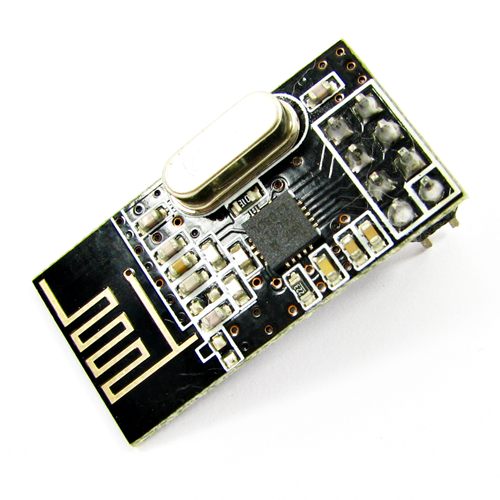
\includegraphics[width=0.5\linewidth]{../../Imagens/nordicc.png}
    \caption{Módulo de Rádio Frequência baseado no \textit{transceiver} da Nordic nRF24L01+}
    \label{Nordic}
  \end{figure}
Módulo de rádio frequência, vide  Fig. \ref{Nordic} obtida de \citeonline{nrf_image}, de baixo custo e consumo cuja faixa de operação situa-se na 
banda S das ondas UHF ( \textit{Ultra 
High Frequency} ), com uma porção dentro da banda ISM \footnote{maiores informações no apêndice}.
Algumas informações técnicas \cite{nRF} de interesse estão listadas abaixo: 
\begin{itemize}
 \item Tensão de alimentação: 1,9V - 3,6V
 \item Antena em circuito impresso do tipo MIFA(\textit{Meandered Inverted-F Antenna}) \cite{MIFA}
 \item Frequência de operação: 2,4GHz - 2,525GHz
 \item Modulação digital do tipo GFSK 
 \item Apresenta até 126 canais de comunicação \footnote{Válido apenas para as taxas de 250kbps e 1 Mbps; a 2Mbps este valor cai à metade, i.e. 63 
canais.}
 \item Taxas de bits: 250kbps, 1Mbps ou 2Mbps
 \item Potências de saída de transmissão: 0dBm, -6dBm, -12dBm e -18dBm
 \item Interface com o microcontrolador por SPI à taxa de até 10Mbps
 \item Pinos de entrada tolerantes a até 5V
 \item 
Pacotes recebidos verificados automaticamente, certificando-se da validade do endereço apontado e legitimando a integridade 
do pacote via CRC(\textit{Cyclic Redundancy Check}) \footnote{Vide apêndice para uma breve explanação sobre CRC}, antes de 
serem movidos às filas de dados recebidos (\textit{RX FIFO})
 \item Receptor envia ao transmissor um pacote de confirmação de recepção dos dados pelo mesmo canal (\textit{acknowledgment packet}).
\end{itemize}

\section{Arduino}
Trata-se de uma plataforma de prototipação eletrônica aberta, i.e. \textit{open-source hardware}, baseada no microcontrolador de 8 bits da Atmel 
ATMega328 \cite{ATMega}, programável via serial (ICSP) através de um microcomputador, por exemplo, por meio do ambiente de desenvolvimento 
\textit{Arduino Software IDE}, \textit{open-source software} e encontra-se no GitHub \cite{ArduSoft}.
Para programar este dispositivo, foi utilizado um módulo baseado na ponte USB-Serial PL-2303, cuja descrição detalhada pode ser encontrada em 
\citeonline{PL2303}.

Algumas informações técnicas \cite{ArduInfo} de interesse estão listadas abaixo: 
\begin{itemize}
 \item Dimensões: 17,78mm x 33mm
 \item Tensão de alimentação recomendável: 5V - 12V
 \item Memória 
 \begin{itemize}
  \item Flash: 32kB 
  \item SRAM: 2kB
  \item EEPROM: 1kB
 \end{itemize}

 \item 20 portas digitais de entrada/saída, das quais 6 podem ser usadas como saídas PWM
 \item 6 portas de entrada analógicas
 \item \textit{clock} de 16MHz
\end{itemize}


\section{Bateria} % TODO
Baterias do tipo LiPo são uma das mais indicadas para veículos elétricos e híbridos, tanto quanto para equipamentos eletrônicos portáteis; no 
entanto, alguns cuidados precisam ser tomados ao manipulá-la por serem sensíveis a sobrecarga ou descarga abrupta.
Logo, por questões de segurança e eficiência é necessário haver um sistema eletrônico para gerenciar a recarga deste dispositivo, o qual monitora a 
tensão de cada uma das células assim como a temperatura em pontos específicos \cite{battery}.
Neste trabalho foi utilizado o carregador IMAX B6-AC para fazer este serviço.
\subsection{\textit{C rate}}
É um parâmetro que descreve a corrente de descarga da bateria em relação à sua capacidade nominal \cite{bateria}.
Vide a Eq. \ref{C rate} para um exemplo ilustrativo baseado na bateria utilizada neste projeto.

\begin{equation}
 \label{C rate}
 30 C = \frac{ I_{descarga} }{ 2.800 mAh} \Rightarrow I_{descarga} \approx 10.7A
\end{equation}

\chapter{Método}
\section{Estratégia \textit{bottom-up}}
A estratégia gerencial e organizacional \textit{bottom-up} foi utilizada no desenvolvimento deste projeto. 
Em função da natureza modular e orientada a comportamentos de arquiteturas reativas \cite{murphy}, a adoção deste método de gerenciamento é quase que 
uma escolha natural.
O robô foi dividido em quatro subsistemas, desenvolvidos e testados separadamente: percepção, locomoção, comunicação e navegação (que, no caso deste 
projeto, consiste no desvio de obstáculos em si). %% TODO citar a arq MOSA aqui pra falar do planejamento??
Nesta fase de implementação,  boas práticas de engenharia de software foram prioridade, buscando uma implementação que 
apresente baixo acoplamento  e alta coesão com a expectativa de desenvolver um código que possa ser facilmente entendido e reutilizado em futuros 
trabalhos afins.
Em seguida se deu a etapa de integração das partes para, a posteriori, serem feitos testes no conjunto, conforme ilustra o diagrama \ref{WBS}.

  \begin{figure}[H] %% TODO certificar se realmente é uma WBS!!!
    \centering
    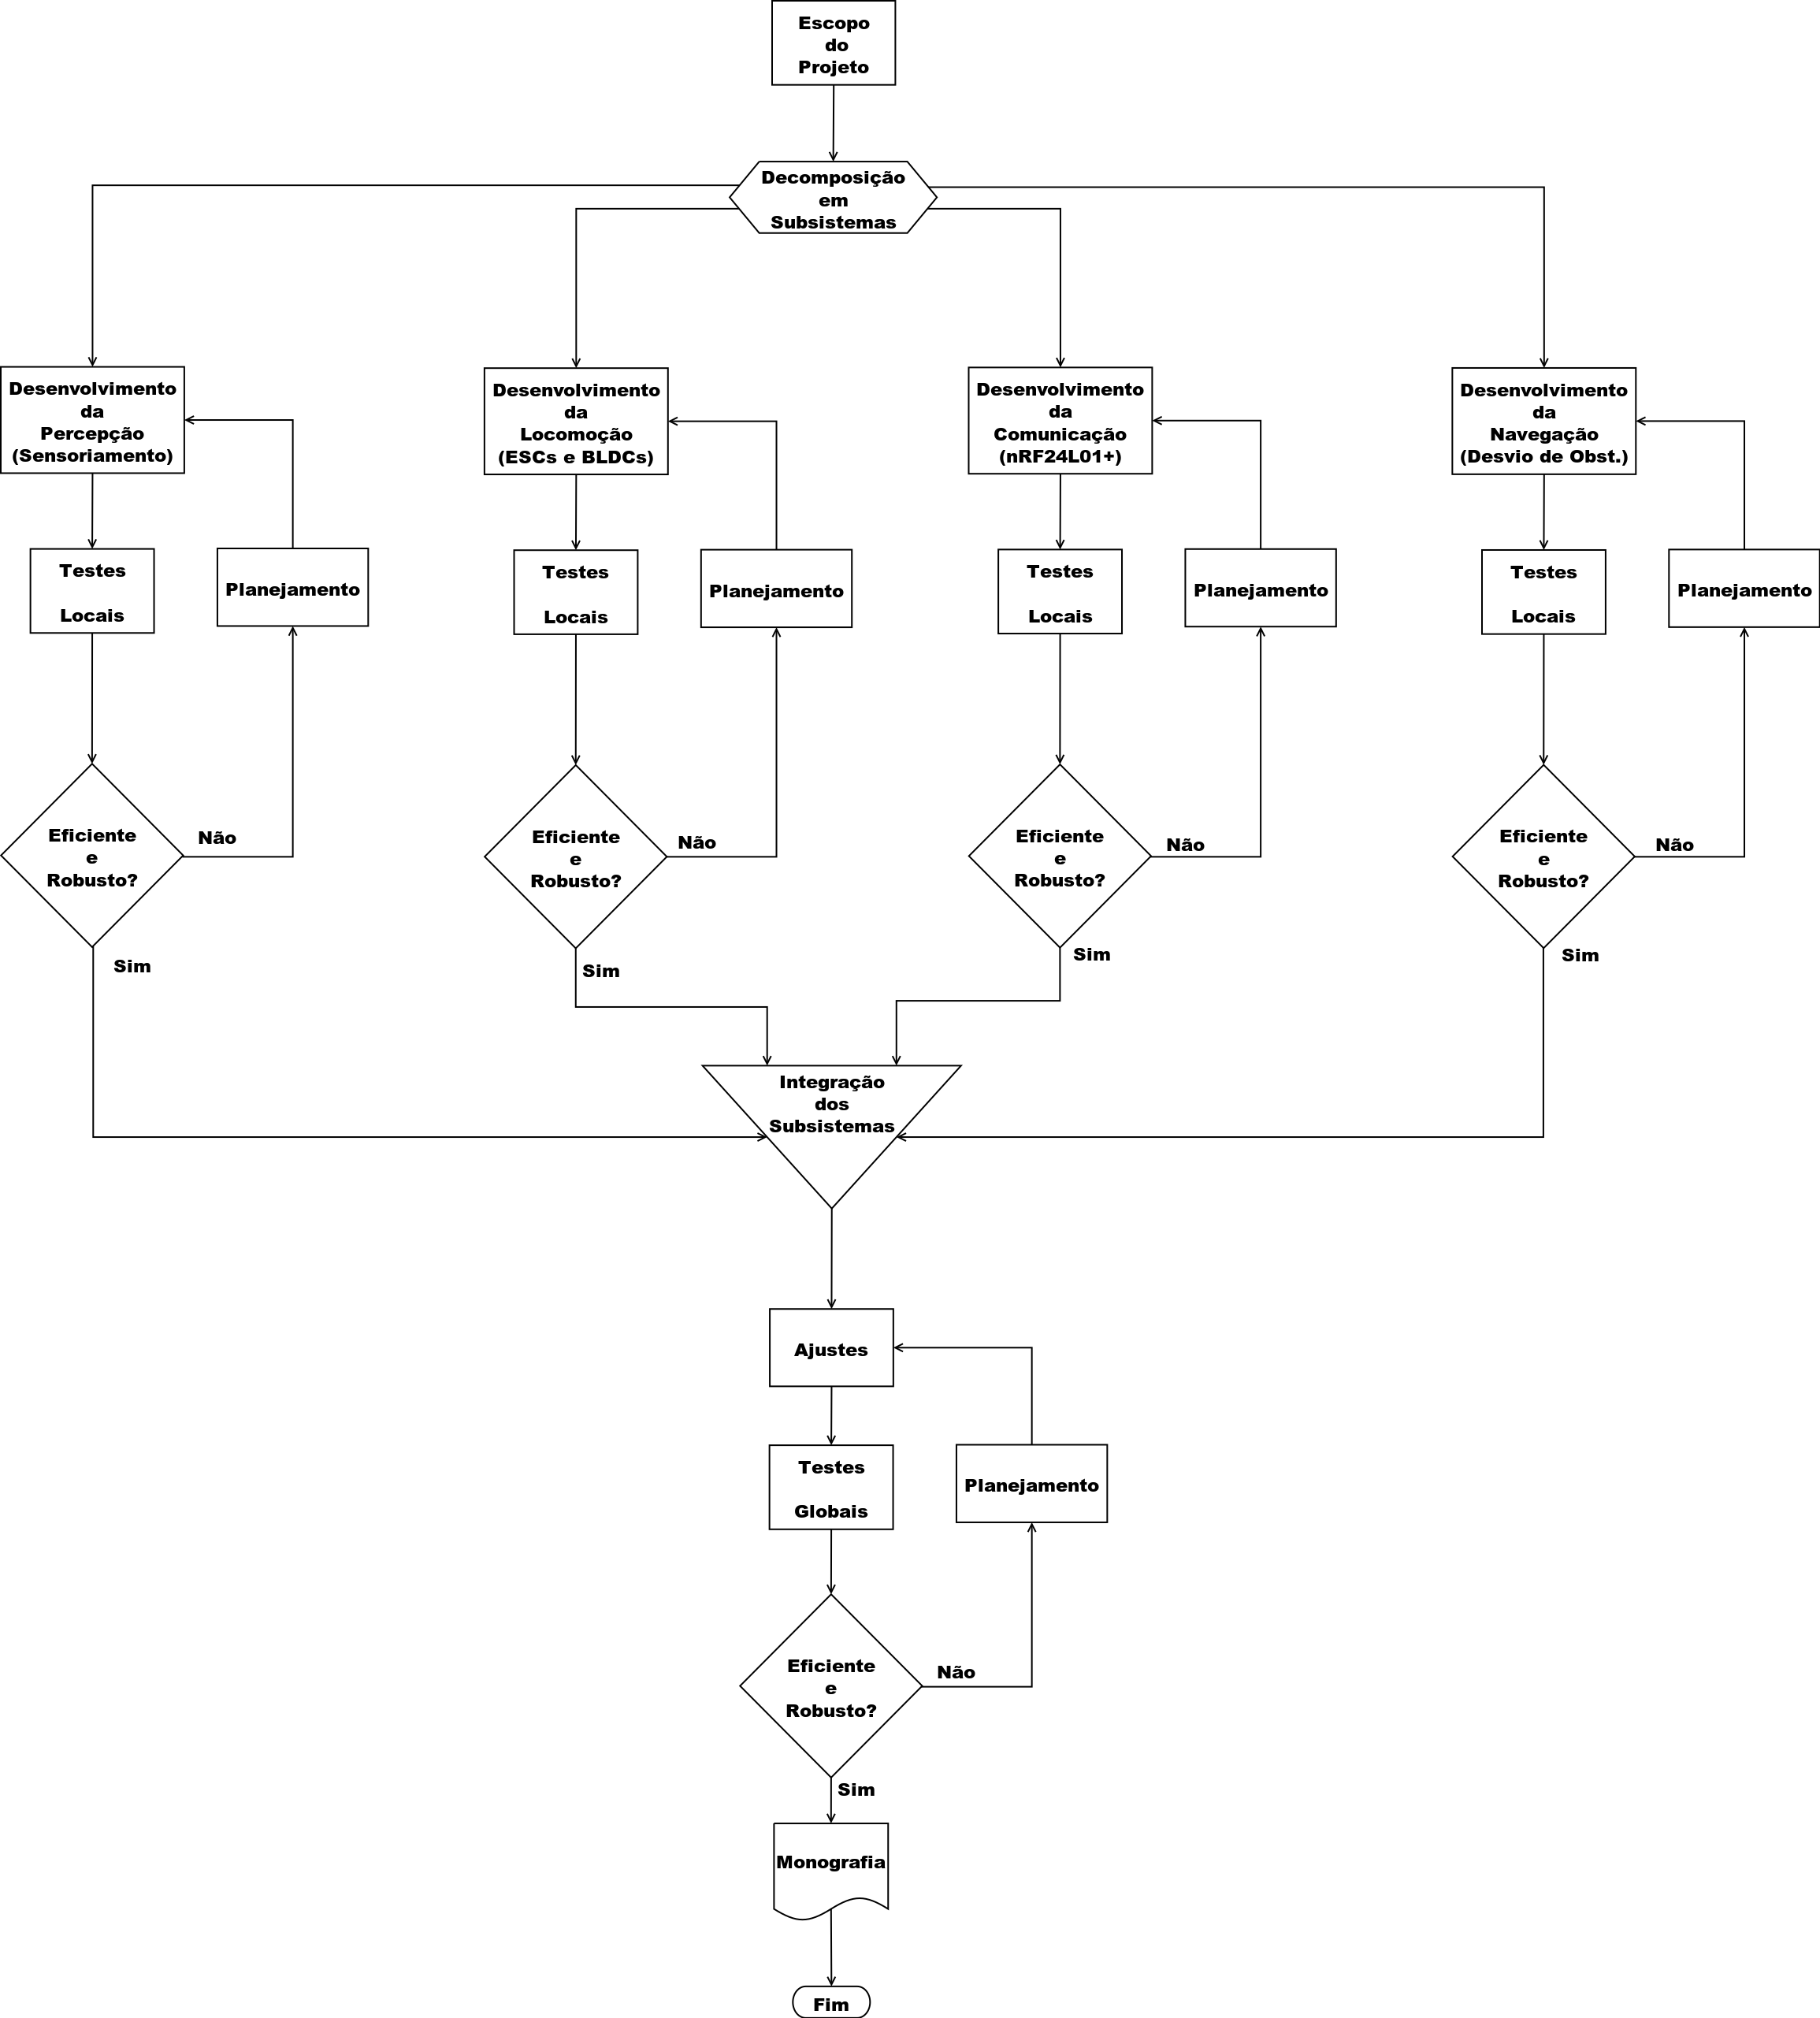
\includegraphics[width= 0.7 \linewidth]{../../Imagens/WBS.png}
    \caption{Estrutura Analítica do Projeto} %% TODO certificar se realmente é uma WBS!!!
    \label{WBS}
  \end{figure}

\section{Arquitetura Reativa} 
% creio não termos implementado uma arquitetura de subsumpção pq o robô apresenta estados internos, como transmissão via RF dos USS quando em modo de 
% navegação e o fato de poder andar caso haja mensagem informando que o SB foi acionado até 500ms antes. 

Optou-se por uma arquitetura de controle fortemente baseada nas informações sensoriais, sem delongas em processamento de sinal para ajustar os dados 
dos sensores a um modelo ou representação de mundo preconcebido. 
A razão dessa escolha é decorrência da necessidade de uma resposta rápida do sistema, vantagem da arquitetura reativa em função da sua simplicidade 
\cite{roseli}.

A latência inerente à obtenção dos dados dos sonares \cite{jones} associada à alta velocidade de operação do robô é a causa desta restrição 
temporal. % TODO não gostei da palavra temporal nesse contexto
Como é imprescindível colher dados do ambiente externo a uma taxa que dê um panorama atualizado do que está se passando ao redor do robô 
\cite{brooks}, reduzir o tempo de resposta do sistema possibilita que o desvio de obstáculos ocorra de maneira mais suave.
Haja vista que se a detecção for feita com antecedência, medidas menos bruscas podem ser adotadas; em contraste com o caso em que a latência é alta a 
ponto de que avpercepção das barreiras no caminho se dê na proximidade do veículo.

Os comportamentos implementados no robô se restringem às diferentes manobras de evasão, adotadas com base na proximidade de obstáculos dos cinco 
sensores, vide Tabela \ref{IA}. Os estímulos reguladores consistem na recepção, via RF, de um comando que incite o robô a navegar e do aval mediante 
recebimento de uma mensagem nos últimos 500ms informando se o botão de segurança foi acionado.
%TODO: as demais funções implementadas podem ser vistas como comportamentos???

\section{Subsistema de Locomoção}
Numa visão geral, temos que o Arduino é responsável por emitir um sinal de controle, modulado em largura de pulso, ao ESC.
Este, por sua vez, é incumbido de energizar os devidos enrolamentos do estator a fim de que o motor BLDC atinja, o mais breve possível, a velocidade 
desejada, expressa pelo sinal de controle. 
Resumidamente: o Arduino comanda, o ESC acata a ordem e conduz o motor a cumprí-la utilizando os recursos da bateria.
O robô apresenta tração dianteira e os motores estão fixos no chassi, logo, faz curvas quando há diferença de velocidade entre os motores.

O código fonte responsável pela produção do pulso PWM nas portas do Arduino foi desenvolvido por Sam Knight e disponibilizado ao público para 
utilização e modificações de qualquer natureza.
Esta biblioteca, denominada PWM, pode ser encontrada no GitHub \cite{pwm_lib}.

%% TODO: terminar isso aqui...

\section{Subsistema de Percepção}
O \textit{software} que manipula os sensores ultrassônicos foi aperfeiçoado aos poucos.
Primeiramente, buscou-se fazer o dispositivo funcionar, utilizando funções prontas e, portanto, não otimizadas de bibliotecas do Arduino.
Em seguida, foi construída a matriz de sensores que, conforme a Fig. \ref{fritzing}, tem o pino de \textit{trigger} comum a todos sonares; no 
entanto, a priori, a leitura dos sonares era feita sequencialmente utilizando o código citado.
O próximo passo, naturalmente, foi fazer com que os cinco sensores fossem lidos paralelamente, aproveitando o fato de todos dispararem juntos, a fim 
de minimizar o tempo de resposta na leitura da matriz.
Em seguida, a fim de reduzir a latência inerente dos sensores ultrassônicos, optou-se por implementar intervalos dinâmicos de medição, isto é, o 
tempo gasto na percepção dependeria do meio no qual o veículo está inserido.  

Foram feitos testes mais rigorosos nessa última configuração com o objetivo de certificar se há de fato a necessidade de estipular um intervalo 
mínimo entre leituras sucessivas dos sonares ou se seria possível que esta latência fosse dinâmica, atrelada ao sensor cujo obstáculo detectado 
encontra-se mais distante.
Em suma, foi verificado se ciclos de leitura menores do que os 60ms sugeridos em \citeonline{HC-SR04} realmente ocasionam aumento na incidência de 
erros 
nas medidas. Os detalhes acerca destes testes constam na seção de resultados.

A decisão de disparar todos os sonares simultaneamente foi feita com o intuito de reduzir o número de portas utilizadas no Arduino, assim como 
aumentar a taxa de obtenção dos dados, i.e. a largura de banda, conforme a terminologia adotada  em \cite{roseli}.
No entanto, as consequências desta deliberação são  severas: agravamento dos fenômenos de \textit{foreshortening} e \textit{crosstalk} 
\cite{2016_artigo_5}. %% TODO: tira o foreshortening daqui??

  \begin{figure}[H]
    \centering
    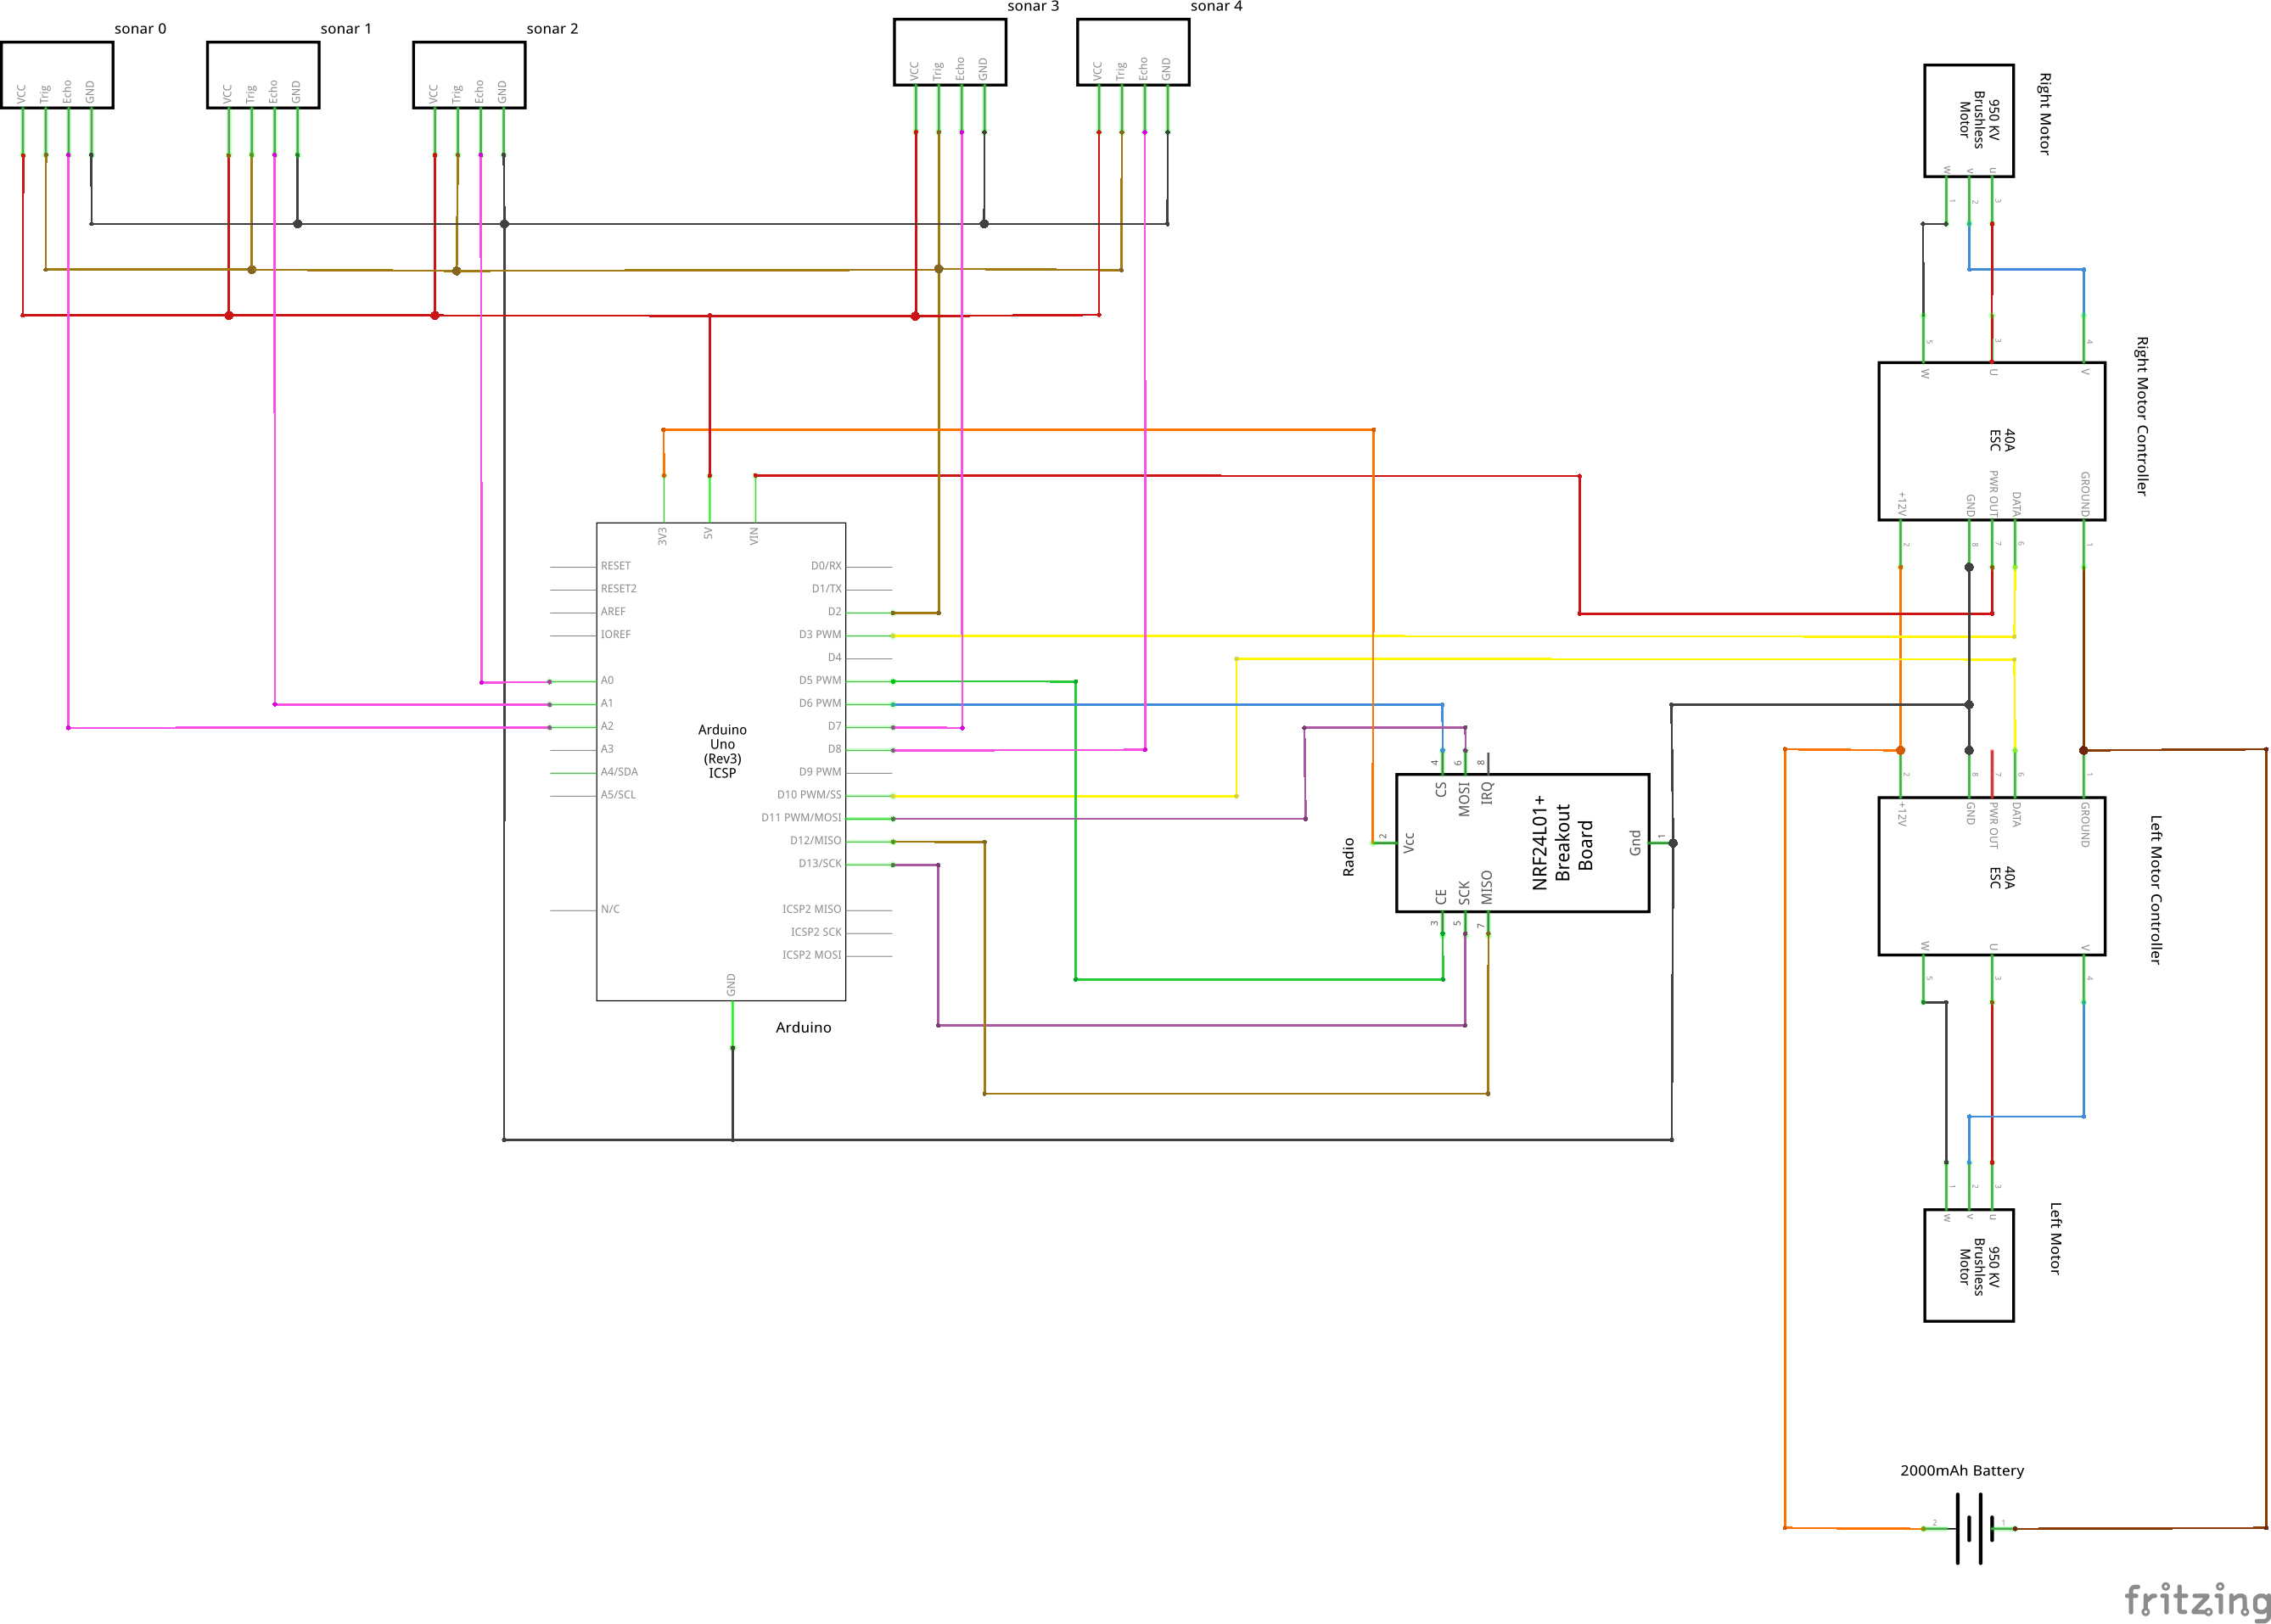
\includegraphics[width= 0.85 \linewidth]{../../Imagens/robot_schem.png}
    \caption{Diagrama Elétrico} %% TODO: é um bom nome??
    \label{fritzing}
  \end{figure}

\section{Subsistema de Comunicação}
Este segmento teve como alicerce a biblioteca denominada RF24, diponível em \cite{nrf_lib}, responsável por todo o controle em baixo nível do 
\textit{transceiver} nRF24L01+.
Foi implementada em C++ e consiste numa única classe, RF24 (vide Fig.\ref{RF24_ClassDiag}), que provê acesso às funcionalidades básicas do 
\textit{transceiver} como controle da potência de transmissão do sinal e escolha do canal a ser utilizado, tanto quanto funções que permitem enviar 
dados por um canal previamente aberto e ler dos canais em que o dispositivo se comporta como receptor; a documentação completa da classe pode ser 
encontrada em \citeonline{RF24_class_doc}.
Assim como todos os códigos de terceiros e programas utilizados nesse projeto, sua utilização é aberta ao público gratuitamente, conforme os termos 
de uso.

Na definição do escopo do projeto, o papel do módulo de radiofrequência seria de simplesmente garantir a segurança e integridade do robô.
Neste caso, uma comunicação \textit{simplex} seria suficiente para cumprir a tarefa.
O módulo transmissor, localizado no acionador remoto, enviava ao robô o nível lógico lido do botão de segurança.
O \textit{transceiver} do robô assumia o papel de receptor e enviava os dados recebidos por comunicação serial ao Arduino, que ordenava a parada dos 
motores caso a mensagem indicasse que o botão estava desligado ou se nenhum pacote fosse detectado num período pré-determinado de 1 segundo.

No entanto, após concluir o sistema de acionamento sem fio, concebeu-se a ideia de sofisticar a utilização do módulo de radiofrequência, 
implementando uma interface de comando capaz de alterar e supervisionar os parâmetros e dados sensoriais do robô, com o intuito de facilitar a etapa 
de testes com o veículo em movimento, objetivando evitar ao máximo a necessidade de reprogramá-lo.

Ao adicionar essa funcionalidade, surge a necessidade de que ambas partes, i.e. robô e sistema de controle remoto, possam receber e enviar 
informações um ao outro.
Como o \textit{transceiver} utilizado tem a funcionalidade de estabelecer comunicação \textit{half-duplex} para cada canal, i.e. bidirecional mas não 
simultaneamente, pois o receptor pode inserir dados no pacote de confirmação de recepção, \textit{acknowledgment packet} \cite{nRF}, e a biblioteca 
RF24 apresenta funções prontas que facilitam o emprego deste recurso, foi possível adicionar essa funcionalidade ao projeto sem a necessidade de 
utilizar dois canais de comunicação.

A interface de comando implementada abrange as seguintes funções:
\begin{itemize}
 \item Ajustar a frequência do PWM de cada um dos motores.
 \item Ajustar a velocidade angular dos motores, que corresponde ao \textit{duty cicle} do sinal de controle, modulado em largura de pulso.
 \item Enviar parâmetros do robô ao controlador remoto: frequência dos PWMs, velocidades dos motores, leituras dos sensores ultrassônicos, 
\textit{status} do botão de segurança de acordo com o veículo.
 \item Energizar os motores na velocidade estipulada enquanto o botão de segurança estiver acionado e não houver obstáculos que representem perigo ao 
robô.
 \item Acionar o sistema de navegação autônoma, também subordinado ao botão de segurança, com tentativas de envio das informações sensoriais e 
comportamentais a cada tomada de decisão do veículo ao controlador remoto sem suspender a movimentação do robô.
 \item Acionar o sistema de navegação autônoma por um número pré-estabelecido de leituras dos sonares, seguido de envio de todos dados coletados ao 
controlador remoto com o robô parado.
\end{itemize}


  \begin{figure}[H]
    \centering
    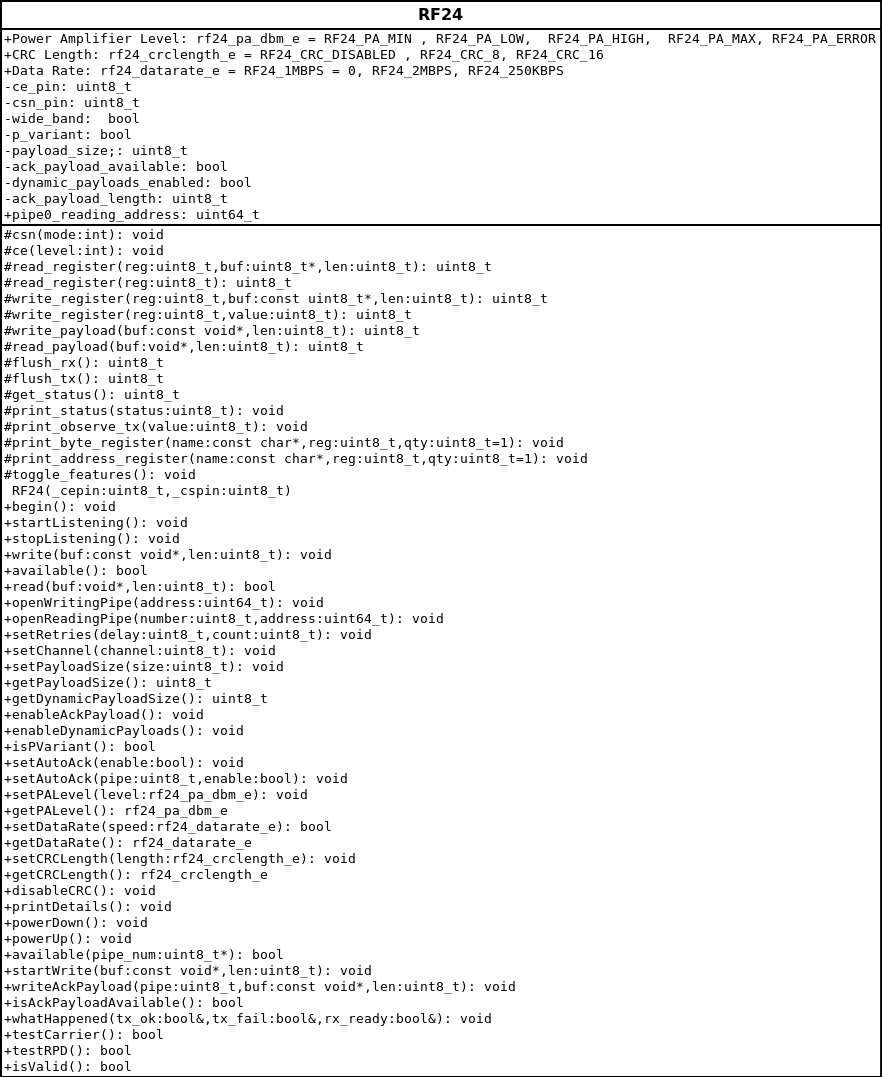
\includegraphics[width=0.5 \linewidth]{../../Imagens/RF24_class.png}
    \caption{Diagrama da Classe RF24} %% TODO certificar se realmente é uma WBS!!!
    \label{RF24_ClassDiag}
  \end{figure}
\section{Subsistema de Navegação} % TODO subsistema ou estratégia de desvio de obstáculos?
Consiste na inteligência  do robô, isto é, trata-se do conjunto de comportamentos adotados pelo veículo, através dos quais ele é capaz de 
desempenhar sua função de desvio de obstáculos. % TODO é realmente necessário falar isso?
Tal qual foi feito em \citeonline{Artigo_3}, a área coberta por um dado sensor ultrassônico foi dividida em três regiões: distante, próxima e perigo.
Quando a leitura de todos os sonares indica região distante, i.e. obstáculos distam mais do que 3 metros, considera-se que o robô 
está seguro e pode andar em velocidade máxima; em futuros trabalhos, corresponderá à situação em que o controle do veículo é cedido ao MOSA.
Caso a medida de algum dos sensores seja menor do que 1 metro - região de perigo - entende-se que o robô está na iminência de uma colisão e deve 
freiar imediatamente.
Quando nenhuma destas situações citadas ocorre, isto é, nenhum dos sonares da matriz está na região de perigo, mas há ao menos um deles que não está 
na região distante, por conseguinte na região próxima, entende-se que há um obstáculo passível de ser contornado.

A estratégia de desvio de obstáculos é semelhante à desenvolvida em \cite{Artigo_1} e define comportamentos bem simples e diretos, como atos reflexos 
nos animais, garantindo rapidez de resposta uma vez que as leituras dos sensores já foram feitas, vide Fig. \ref{ObstAvoid}.
Analisa-se cada um dos cinco sonares quanto à região em que se encontra a barreira identificada: 0 para região distante e 1, próxima;
cada uma das 32 combinações possíveis apresenta um comportamento correspondente: seguir em frente, fazer uma curva aberta, moderada ou brusca.
Na Tabela \ref{IA} utiliza-se \textquoteleft E\textquoteright{} e  \textquoteleft D\textquoteright{} para designar curvas à esquerda e direita, 
respectivamente; enquanto os índices \textquoteleft L\textquoteright{},  \textquoteleft M\textquoteright{} e \textquoteleft F\textquoteright{} 
caracterizam o quão acentuada vai ser a curva: leve, moderada ou forte. % tirar isso daqui e colocar legenda na tabela. 

  \begin{figure}[H]
    \centering
    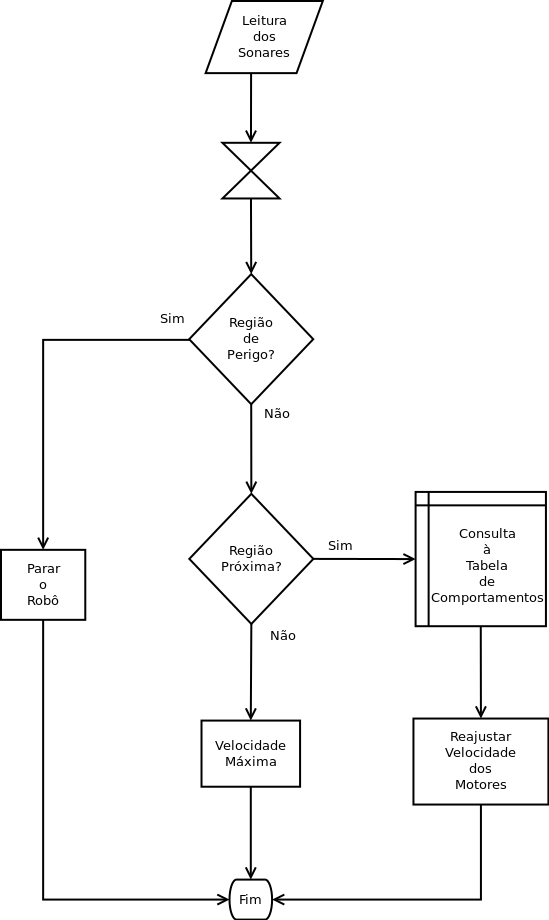
\includegraphics[width=0.5 \linewidth]{../../Imagens/ObstAvoid.png}
    \caption{Fluxograma da Rotina de Desvio de Obstáculos}
    \label{ObstAvoid}
  \end{figure}
  
\section{Integração dos Subsistemas}
Assim que todos os subsistemas foram implementados, testados e operavam isoladamente de maneira satisfatória, foram feitos testes no conjunto, que 
indicaram novos problemas a serem tratados. 
A maioria deles de ordem prática e facilmente contornáveis, no entanto um é digno de nota, pois implicou em uma mudança na disposição física dos 
componentes do veículo que acabou não solucionando o problema. Maiores detalhes, vide seção de Resultados.
\chapter{Resultados}

\section{Testes Unitários}

\subsection{Intervalo de Medição Dinâmico}
A fim de verificar a viabilidade de impregar-se intervalos dinâmicos na percepão do veículo, este foi disposto em diferentes posições nas quais todos 
os sonares apresentavam obstáculos visíveis, foram realizadas medições dinâmicas e estáticas, esta última com três intervalos distintos: 30ms, 45ms e 
60ms. Em cada uma das medições foram armazenadas 150 leituras ininterruptas armazenadas em um \textit{buffer} local que, ao ser preenchido, cessava 
o acionamento dos sonares e imprimia os dados via interface serial antes de começar a próxima medição. 
Nos dados obtidos em cada uma dessas medições foram feitos cálculos de média e desvio padrão sujos e limpos\footnote{foram consideradas medidas 
limpas aquelas cuja métrica foi calculada descartando-se as leituras em que o respectivo sonar não encontrou o obstáculo}, contagem dos resultados 
que desviassem em mais do que quatro vezes o desvio padrão em relação à média limpa das leituras.

\subsection{Leituras Espúrias nos Sonares}
%% testes feitos com o veículo parado nas quais surgiam valores conflitantes
Ao serem feitos testes unitários no \textit{software} de controle dos sensores ultrassônicos, notou-se a existência de leituras espúrias, sobretudo 
em condições em que não havia obstáculos dentre da região visível do dispositivo.
A fim de documentar o problema, posiciou-se o veículo num ângulo e distância conhecidos em relação a um obstáculo para em seguida medir as respostas 
dos sonares; foram feitos diversos testes variando o ângulo e a distância dos obstáculos, incluindo o caso de não haver obstáculos dentro do 
alcance de detecção dos sensores ultrassônicos, variou-se também o \textit{blanking time}.
Os valores coletados constam nas Tabelas \ref{espurias-1}, \ref{espurias-2}.

Podemos notar que não há uma correlação entre o \textit{dead time} e a aparição das leituras espúrias, o que motivou a adoção de intervalos dinâmicos 
de leitura, isto é, o \textit{blanking time} corresponde ao intervalo do sonar que demorou mais a receber uma resposta no pino de \textit{echo} ou um 
 valor máximo pré-determinado, caso não haja obstáculos ao alcance de algum deles.
A solução concebida para remediar este problema foi basear o comportamento a ser adotado na média aritmética das últimas 5 leituras, excluindo os 
valores extremos.

\section{Testes de Integração}
\subsection{Interferência dos BLDC nos Sonares}
Notou-se que em determinadas condições o robô ia de encontro ao obstáculo ao invés de efetuar o desvio. 
Após serem analisados os dados dos sensores nessas circunstâncias, observou-se a existência de ruídos em sensores específicos, que causavam a adoção 
destes comportamentos errados.

Ao perceber o problema, novos testes foram engendrados a fim de descobrir a natureza da falha.
As hipóteses concebidas eram as seguintes: \textit{crosstalk}, curto circuito entre pinos do Arduino, falha na lógica do \textit{software} ou 
interferência dos motores nos sensores.

Para eliminar a possibilidade de que uma das portas da placa de prototipação estivesse interferindo na outra de alguma maneira, mudou-se a 
ligação dos sensores ultrassônicos e o problema se manteve.
O mesmo foi feito no \textit{software}, i.e. foi alterada a disposição dos sensores ultrassônicos no código. 
Especificamente falando, foram trocados os parâmetros que correlacionam a ligação física do pino de \textit{echo} dos dispositivos à sua variável 
correspondente na matriz de estruturas do tipo \textit{sensor\_t}, denominada no programa por USS, e, mais uma vez, o defeito persistiu.
Adicionalmente a essa modificação no \textit{software}, foram feitas medições com os motores desligados, nas quais a falha em questão não ocorreu, 
evidenciando que a natureza do problema não era do código.

O teste seguinte consistiu em desacoplar os sensores ultrassônicos da carcaça do veículo e ligar os motores com os sonares sendo segurados na mão, o 
no resultado observou-se a desaparição das leituras espúrias, confirmando a hipótese de que os BLDC causavam a distorção na percepção do robô.
Em vista disso, supôs-se que a natureza da interferência seria em razão da proximidade entre os dispositivos, como interferência eletromagnética nos 
pinos de \textit{echo} dos sonares ou então de ondas acústica na banda de funcionamento do sensor, e optou-se por erguer os sensores a uma altura 
na qual não houvesse interferência suficiente a ponto de provocar erros de medição.

Após terem sido feitas as devidas modificações, foi engendrado um novo teste a fim de constatar se com a nova disposição o problema havia sido 
sanado: cada uma das combinações de velocidades dos motores foi mantida por dez segundos enquanto os sonares faziam as medições.
Os dados obtidos, vide Tabela \ref{tabela-interf}, apontaram que o problema persistia; enquanto era realizado o teste, notou-se que os fios oscilavam
 em decorrência da vibração dos motores, o que levou a cogitar a hipótese de que essa seria de fato a natureza da interferência entre os sensores 
ultrassônicos e os motores.

%%% ----------------------------------------------------------------------------------------------------------------------------------------------
\cite{jones}(página 149) vibração residual do trigger pode causar falsas leituras no echo, talvez esse seja o problema no caso de detecções dinâmicas 
deixado de lado.

\cite{siegwart} (páginas 126-127) talvez estendendo o \textit{blanking time} consigamos manter as detecções dinâmicas. Como fazer isso:
\begin{itemize}
 \item colocar um delay antes de entrar no loop
 \item mexer diretamente no myPulsein() para garantir medidas abaixo de 5 cm não sejam processadas trabalhando nos IFs. 
\end{itemize}

 While comparison of consecutive readings is an efficient way for rejecting external
 erroneous readings, it is unsuitable for reducing crosstalk. \cite{2016_artigo_1}


\chapter{Conclusão}

% ----------------------------------------------------------
% ELEMENTOS PÓS-TEXTUAIS
% ----------------------------------------------------------
\postextual
% ----------------------------------------------------------

% ----------------------------------------------------------
% Referências bibliográficas
% ----------------------------------------------------------
\bibliography{../Bibliografia/bibliografia.bib}

% ----------------------------------------------------------
% Glossário
% ----------------------------------------------------------
%
% Consulte o manual da classe abntex2 para orientações sobre o glossário.
%
%\glossary

% ----------------------------------------------------------
% Apêndices
% ----------------------------------------------------------

% ---
% Inicia os apêndices
% ---
\begin{apendicesenv}
% Imprime uma página indicando o início dos apêndices
 \partapendices
\chapter{Apêndices}

\section{Diagrama da Classe RF24}
  \begin{figure}[!htb]
    \centering
    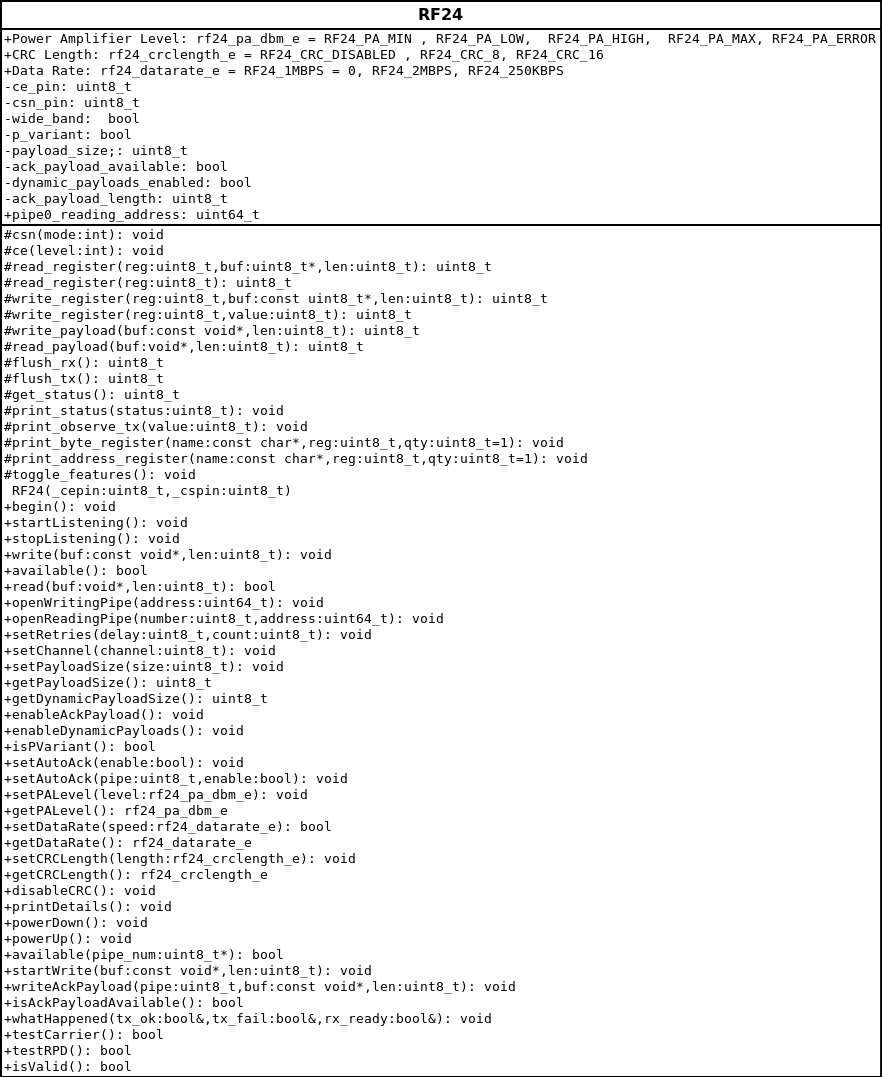
\includegraphics[width=\linewidth]{../../Imagens/RF24_class.png}
    \caption{Diagrama da Classe RF24} %% TODO certificar se realmente é uma WBS!!!
    \label{RF24_ClassDiag}
  \end{figure}

\section{Estrutura Analítica do Projeto}
  \begin{figure}[!htb] %% TODO certificar se realmente é uma WBS!!!
    \centering
    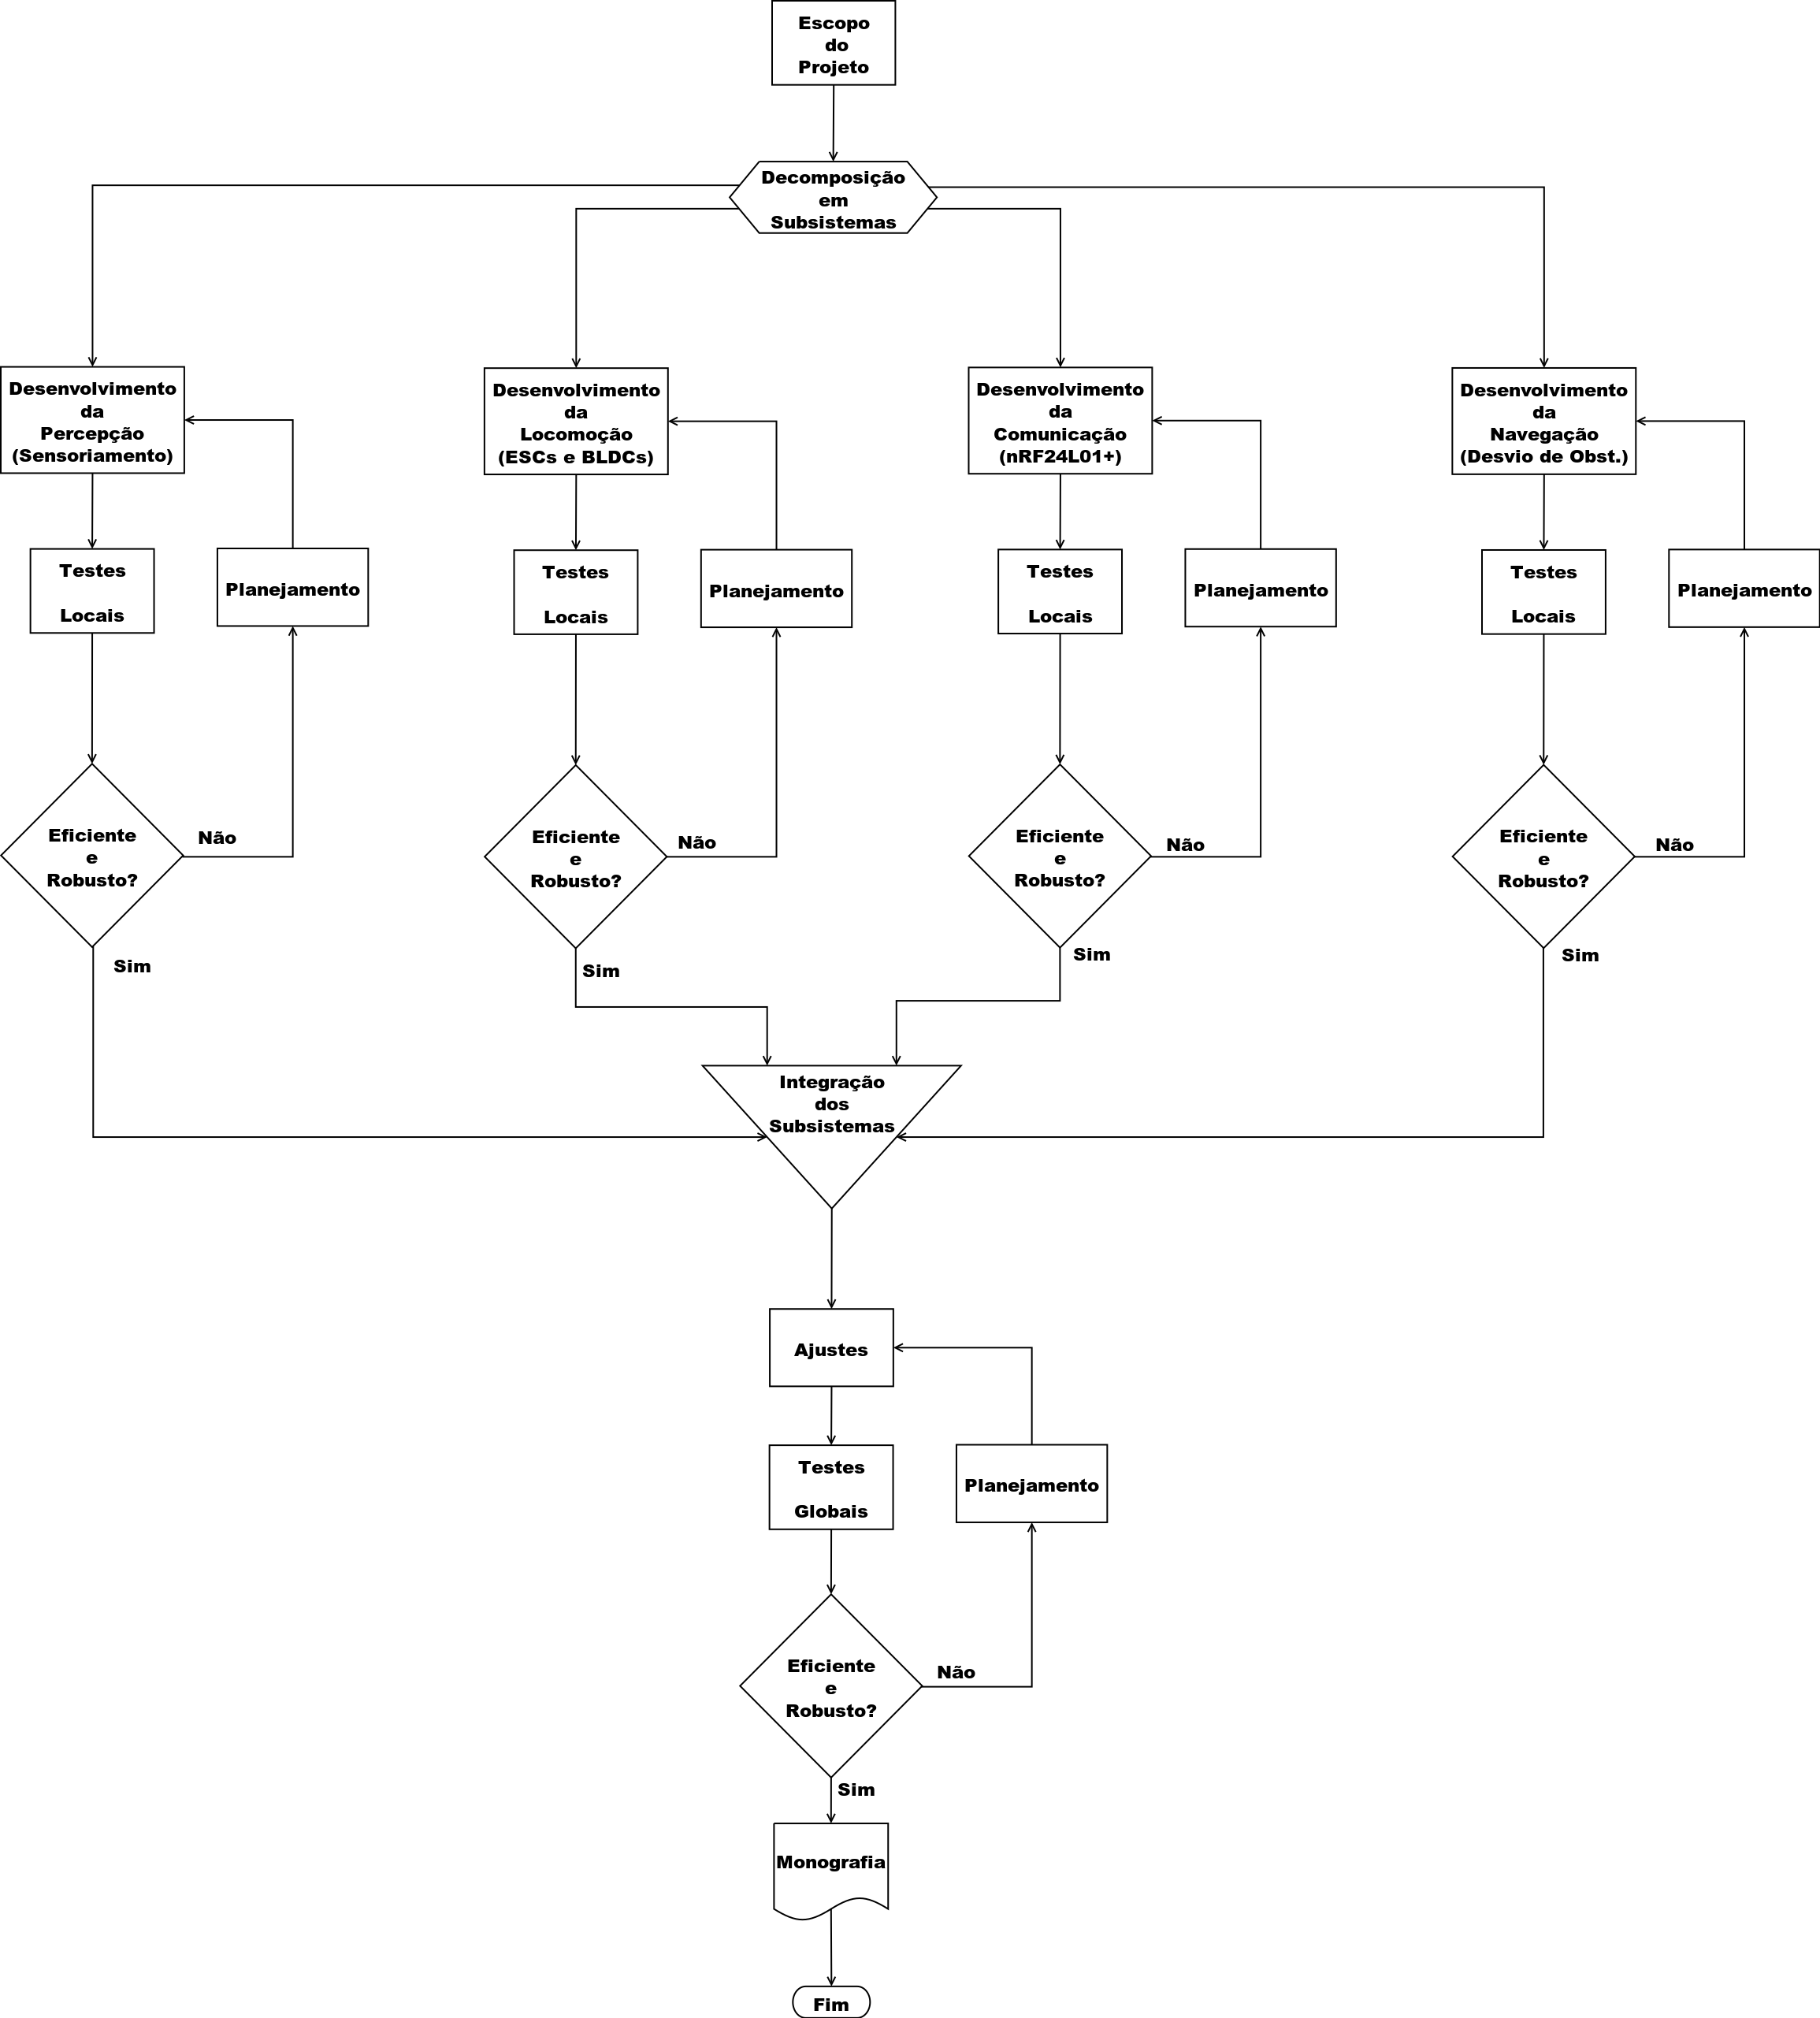
\includegraphics[width=\linewidth]{../../Imagens/WBS.png}
    \caption{Estrutura Analítica do Projeto} %% TODO certificar se realmente é uma WBS!!!
    \label{WBS}
  \end{figure}
  
\section{Esquemático do Robô}
  \begin{figure}[!htb]
    \centering
    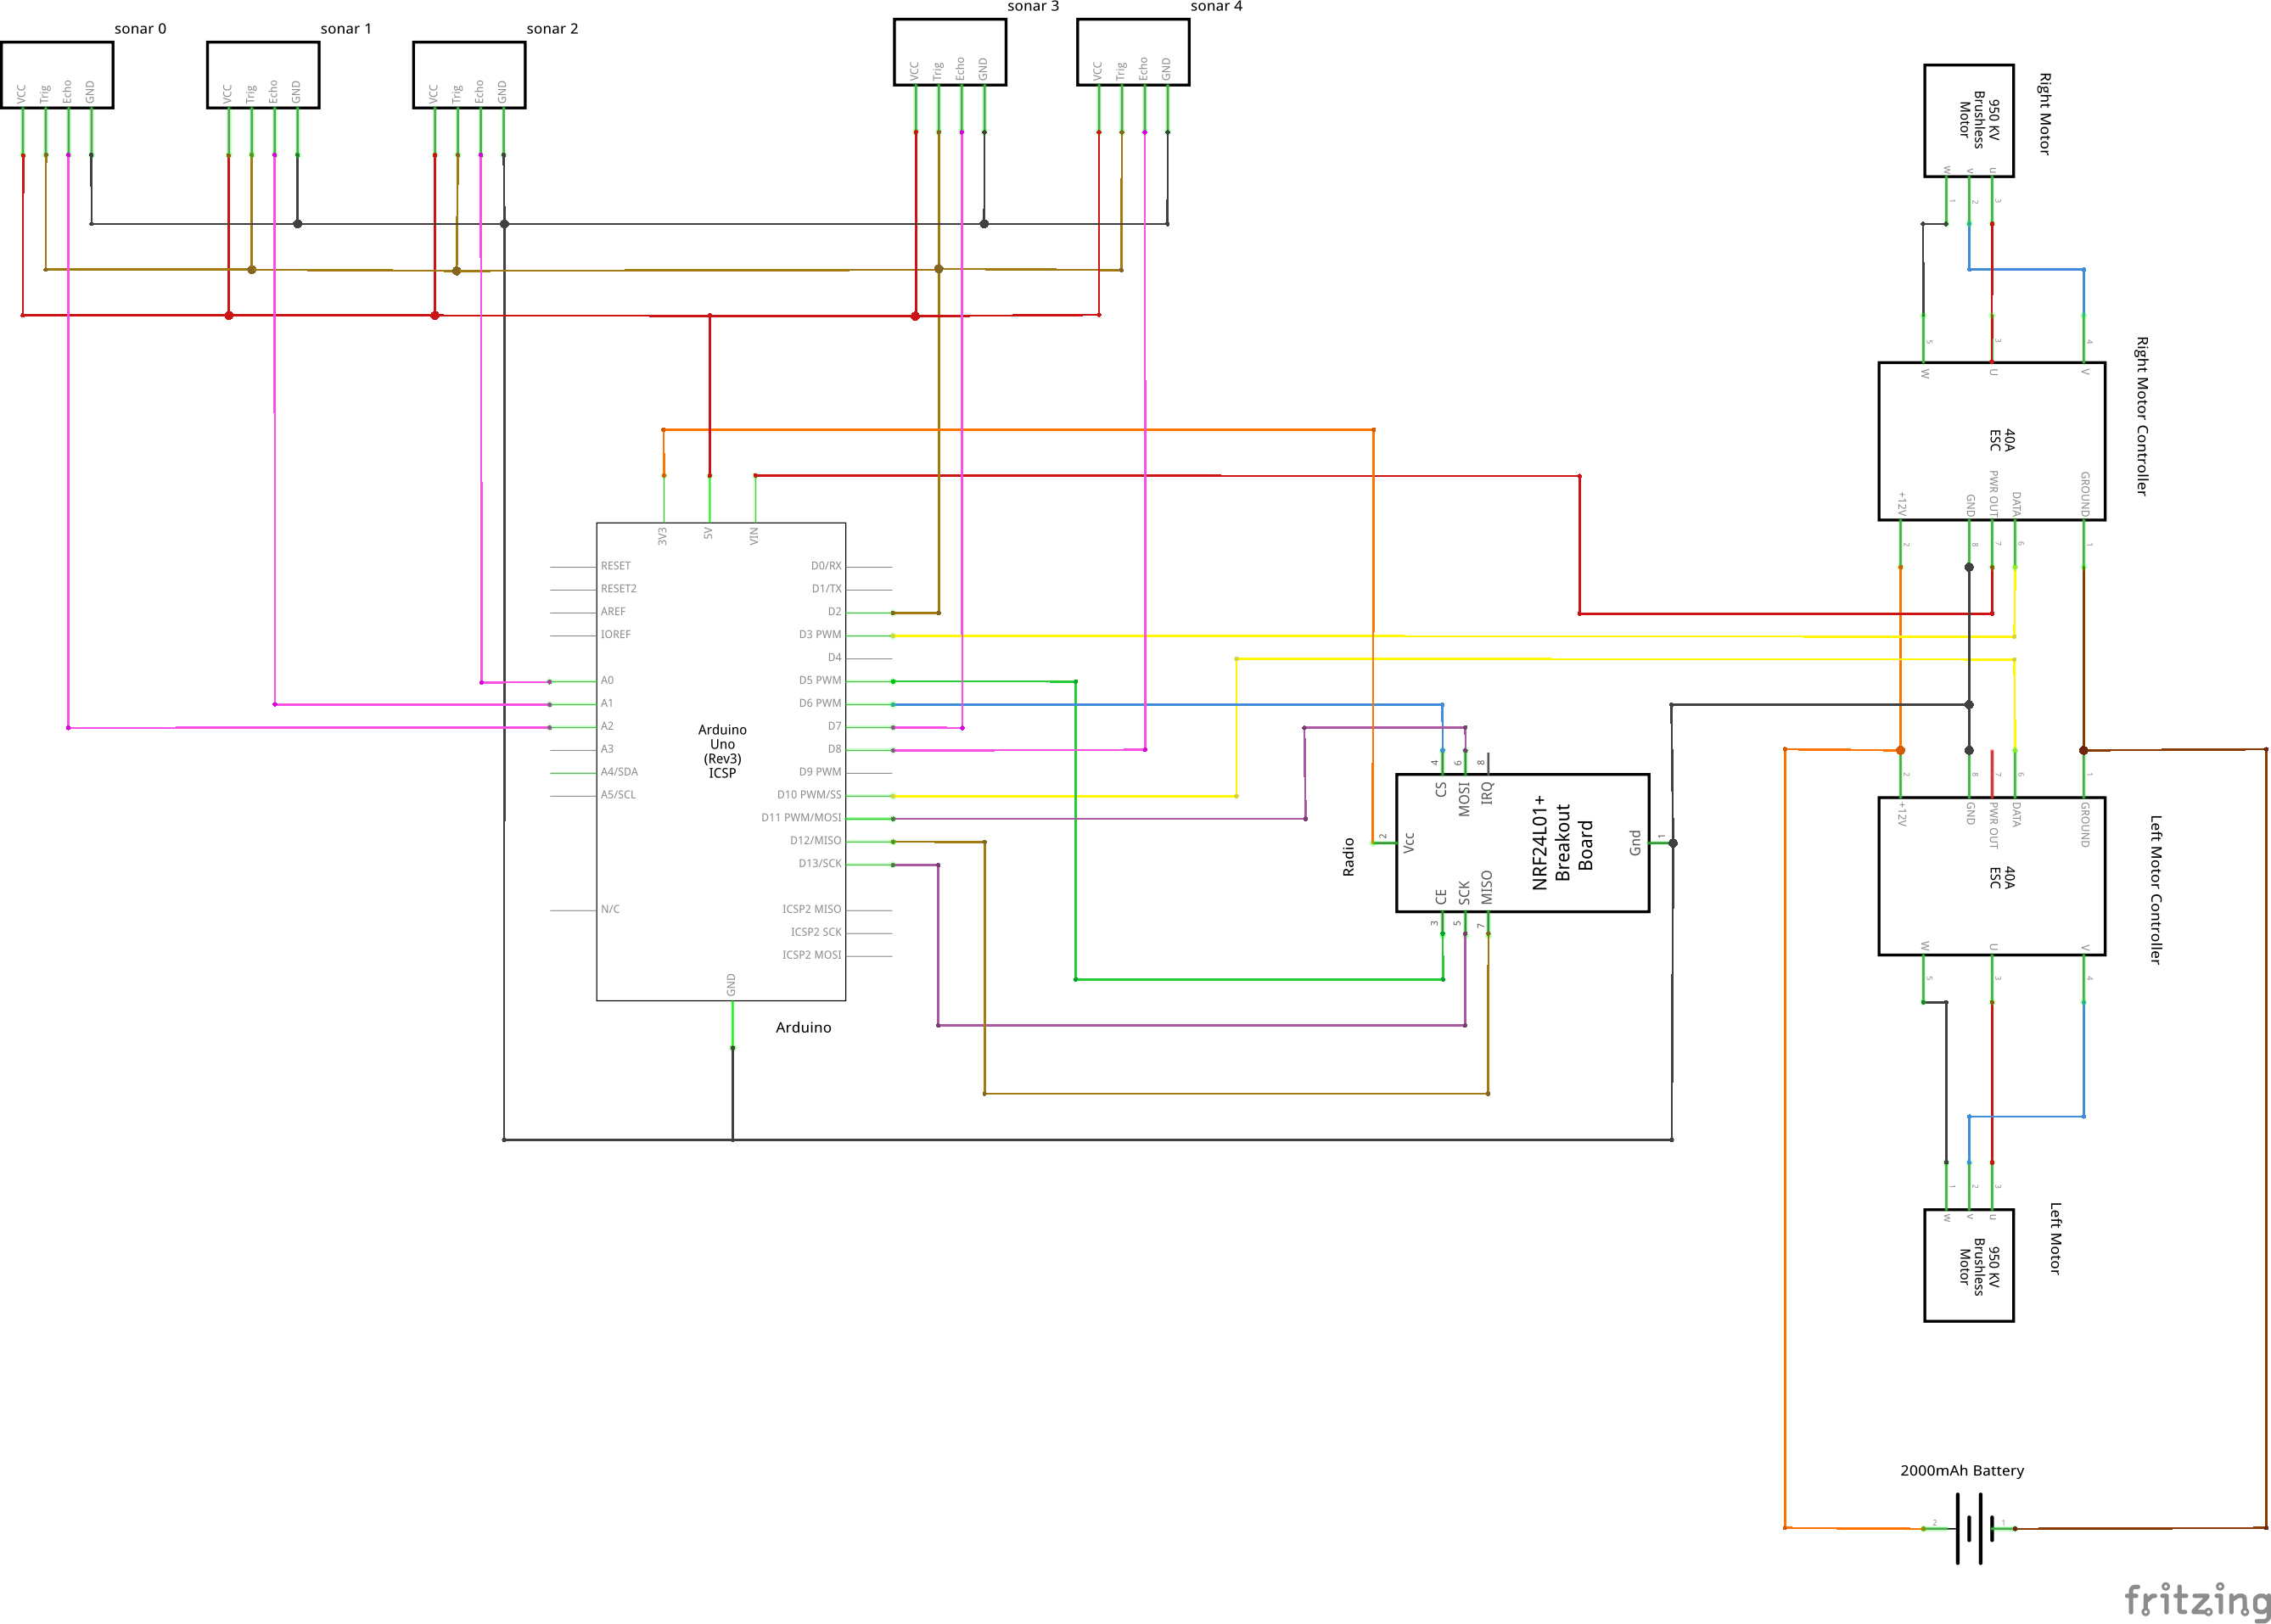
\includegraphics[width=\linewidth]{../../Imagens/robot_schem.png}
    \caption{Diagrama Elétrico} %% TODO: é um bom nome??
    \label{fritzing}
  \end{figure}
  
% TODO desatualizada!!!!
\section{Tabela} % TODO desatualizada!!!!
% TODO desatualizada!!!!
\begin{table}[!htb]
\centering
\caption{}
\label{IA}
\begin{tabular}{|ccccc|c|}
\hline
{\color[HTML]{00009B} \textbf{$USS_0$}} & {\color[HTML]{00009B} \textbf{$USS_1$}} & {\color[HTML]{00009B} \textbf{$USS_2$}} & 
{\color[HTML]{00009B} \textbf{$USS_3$}} & {\color[HTML]{00009B} \textbf{$USS_4$}} & {\color[HTML]{FE0000} \textbf{Ação}} \\ 
\hline
{\color[HTML]{00009B} 0}                                     & {\color[HTML]{00009B} 0}                                    & {\color[HTML]{00009B} 0}  
                                  & {\color[HTML]{00009B} 0}                                    & {\color[HTML]{00009B} 1}                             
       & {\color[HTML]{FE0000} $E_L$}                                     \\ \hline
{\color[HTML]{00009B} 0}                                     & {\color[HTML]{00009B} 0}                                    & {\color[HTML]{00009B} 0}  
                                  & {\color[HTML]{00009B} 1}                                    & {\color[HTML]{00009B} 0}                             
       & {\color[HTML]{FE0000} $E_M$}                                     \\ \hline
{\color[HTML]{00009B} 0}                                     & {\color[HTML]{00009B} 0}                                    & {\color[HTML]{00009B} 0}  
                                  & {\color[HTML]{00009B} 1}                                    & {\color[HTML]{00009B} 1}                             
       & {\color[HTML]{FE0000} $E_M$}                                     \\ \hline
{\color[HTML]{00009B} 0}                                     & {\color[HTML]{00009B} 0}                                    & {\color[HTML]{00009B} 1}  
                                  & {\color[HTML]{00009B} 0}                                    & {\color[HTML]{00009B} 0}                             
       & {\color[HTML]{FE0000} $E_F$}                                     \\ \hline
{\color[HTML]{00009B} 0}                                     & {\color[HTML]{00009B} 0}                                    & {\color[HTML]{00009B} 1}  
                                  & {\color[HTML]{00009B} 0}                                    & {\color[HTML]{00009B} 1}                             
       & {\color[HTML]{FE0000} $E_F$}                                     \\ \hline
{\color[HTML]{00009B} 0}                                   & {\color[HTML]{00009B} 0}                                    & {\color[HTML]{00009B} 1}    
                                & {\color[HTML]{00009B} 1}                                    & {\color[HTML]{00009B} 0}                               
     & {\color[HTML]{FE0000} $E_F$}                                     \\ \hline
{\color[HTML]{00009B} 0}                                    & {\color[HTML]{00009B} 0}                                  & {\color[HTML]{00009B} 1}     
                               & {\color[HTML]{00009B} 1}                                    & {\color[HTML]{00009B} 1}                                
    & {\color[HTML]{FE0000} $E_F$}                                     \\ \hline
{\color[HTML]{00009B} 0}                                     & {\color[HTML]{00009B} 1}                                    & {\color[HTML]{00009B} 0}  
                                & {\color[HTML]{00009B} 0}                                    & {\color[HTML]{00009B} 0}                               
     & {\color[HTML]{FE0000} $D_M$}                                     \\ \hline
{\color[HTML]{00009B} 0}                                    & {\color[HTML]{00009B} 1}                                    & {\color[HTML]{00009B} 0}   
                                 & {\color[HTML]{00009B} 0}                                 & {\color[HTML]{00009B} 1}                                 
   & {\color[HTML]{FE0000} $D_M$}                                     \\ \hline
{\color[HTML]{00009B} 0}                                    & {\color[HTML]{00009B} 1}                                    & {\color[HTML]{00009B} 0}   
                                 & {\color[HTML]{00009B} 1}                                    & {\color[HTML]{00009B} 0}                              
      & {\color[HTML]{FE0000} $E_F$}                                     \\ \hline
{\color[HTML]{00009B} 0}                                    & {\color[HTML]{00009B} 1}                                    & {\color[HTML]{00009B} 0}   
                                 & {\color[HTML]{00009B} 1}                                    & {\color[HTML]{00009B} 1}                              
      & {\color[HTML]{FE0000} $E_M$}                                  \\ \hline
{\color[HTML]{00009B} 0}                                     & {\color[HTML]{00009B} 1}                                    & {\color[HTML]{00009B} 1}  
                                  & {\color[HTML]{00009B} 0}                                    & {\color[HTML]{00009B} 0}                             
       & {\color[HTML]{FE0000} $D_F$}                                     \\ \hline
{\color[HTML]{00009B} 0}                                     & {\color[HTML]{00009B} 1}                                    & {\color[HTML]{00009B} 1}  
                                  & {\color[HTML]{00009B} 0}                                    & {\color[HTML]{00009B} 1}                             
       & {\color[HTML]{FE0000} $E_F$}                                     \\ \hline
{\color[HTML]{00009B} 0}                                     & {\color[HTML]{00009B} 1}                                    & {\color[HTML]{00009B} 1}  
                                  & {\color[HTML]{00009B} 1}                                    & {\color[HTML]{00009B} 0}                             
       & {\color[HTML]{FE0000} $E_F$}                                     \\ \hline
{\color[HTML]{00009B} 0}                                     & {\color[HTML]{00009B} 1}                                    & {\color[HTML]{00009B} 1}  
                                  & {\color[HTML]{00009B} 1}                                    & {\color[HTML]{00009B} 1}                             
       & {\color[HTML]{FE0000} $E_F$}                                     \\ \hline
{\color[HTML]{00009B} 1}                                     & {\color[HTML]{00009B} 0}                                    & {\color[HTML]{00009B} 0}  
                                  & {\color[HTML]{00009B} 0}                                    & {\color[HTML]{00009B} 0}                             
       & {\color[HTML]{FE0000} $D_L$}                                     \\ \hline
{\color[HTML]{00009B} 1}                                     & {\color[HTML]{00009B} 0}                                    & {\color[HTML]{00009B} 0}  
                                  & {\color[HTML]{00009B} 0}                                    & {\color[HTML]{00009B} 1}                             
       & {\color[HTML]{FE0000} Frente}                                     \\ \hline
{\color[HTML]{00009B} 1}                                     & {\color[HTML]{00009B} 0}                                    & {\color[HTML]{00009B} 0}  
                                  & {\color[HTML]{00009B} 1}                                    & {\color[HTML]{00009B} 0}                             
       & {\color[HTML]{FE0000} $E_M$}                                     \\ \hline
{\color[HTML]{00009B} 1}                                     & {\color[HTML]{00009B} 0}                                    & {\color[HTML]{00009B} 0}  
                                  & {\color[HTML]{00009B} 1}                                    & {\color[HTML]{00009B} 1}                             
       & {\color[HTML]{FE0000} $E_M$}                                     \\ \hline
{\color[HTML]{00009B} 1}                                     & {\color[HTML]{00009B} 0}                                    & {\color[HTML]{00009B} 1}  
                                  & {\color[HTML]{00009B} 0}                                    & {\color[HTML]{00009B} 0}                             
       & {\color[HTML]{FE0000} $D_F$}                                     \\ \hline
{\color[HTML]{00009B} 1}                                     & {\color[HTML]{00009B} 0}                                    & {\color[HTML]{00009B} 1}  
                                  & {\color[HTML]{00009B} 0}                                    & {\color[HTML]{00009B} 1}                             
       & {\color[HTML]{FE0000} $E_F$}                                     \\ \hline
{\color[HTML]{00009B} 1}                                     & {\color[HTML]{00009B} 0}                                    & {\color[HTML]{00009B} 1}  
                                  & {\color[HTML]{00009B} 1}                                    & {\color[HTML]{00009B} 0}                             
       & {\color[HTML]{FE0000} $E_F$}                                     \\ \hline
{\color[HTML]{00009B} 1}                                     & {\color[HTML]{00009B} 0}                                    & {\color[HTML]{00009B} 1}  
                                  & {\color[HTML]{00009B} 1}                                    & {\color[HTML]{00009B} 1}                             
       & {\color[HTML]{FE0000} $E_F$}                                     \\ \hline
{\color[HTML]{00009B} 1}                                     & {\color[HTML]{00009B} 1}                                    & {\color[HTML]{00009B} 0}  
                                  & {\color[HTML]{00009B} 0}                                    & {\color[HTML]{00009B} 0}                             
       & {\color[HTML]{FE0000} $D_M$}                                     \\ \hline
{\color[HTML]{00009B} 1}                                     & {\color[HTML]{00009B} 1}                                    & {\color[HTML]{00009B} 0}  
                                  & {\color[HTML]{00009B} 0}                                    & {\color[HTML]{00009B} 1}                             
       & {\color[HTML]{FE0000} $D_M$}                                     \\ \hline
{\color[HTML]{00009B} 1}                                     & {\color[HTML]{00009B} 1}                                    & {\color[HTML]{00009B} 0}  
                                  & {\color[HTML]{00009B} 1}                                    & {\color[HTML]{00009B} 0}                             
       & {\color[HTML]{FE0000} $D_M$}                                     \\ \hline
{\color[HTML]{00009B} 1}                                     & {\color[HTML]{00009B} 1}                                    & {\color[HTML]{00009B} 0}  
                                  & {\color[HTML]{00009B} 1}                                    & {\color[HTML]{00009B} 1}                             
       & {\color[HTML]{FE0000} Frente}                                     \\ \hline
{\color[HTML]{00009B} 1}                                     & {\color[HTML]{00009B} 1}                                    & {\color[HTML]{00009B} 1}  
                                  & {\color[HTML]{00009B} 0}                                    & {\color[HTML]{00009B} 0}                             
       & {\color[HTML]{FE0000} $D_F$}                                     \\ \hline
{\color[HTML]{00009B} 1}                                     & {\color[HTML]{00009B} 1}                                    & {\color[HTML]{00009B} 1}  
                                  & {\color[HTML]{00009B} 0}                                    & {\color[HTML]{00009B} 1}                             
       & {\color[HTML]{FE0000} $D_F$}                                     \\ \hline
{\color[HTML]{00009B} 1}                                     & {\color[HTML]{00009B} 1}                                    & {\color[HTML]{00009B} 1}  
                                  & {\color[HTML]{00009B} 1}                                    & {\color[HTML]{00009B} 0}                             
       & {\color[HTML]{FE0000} $D_F$}                                     \\ \hline
{\color[HTML]{00009B} 1}                                     & {\color[HTML]{00009B} 1}                                    & {\color[HTML]{00009B} 1}  
                                  & {\color[HTML]{00009B} 1}                                    & {\color[HTML]{00009B} 1}                             
       & {\color[HTML]{FE0000} $E_F$}                                    \\ \hline

\end{tabular}
\end{table}

\section{Fluxograma da Rotina de Desvio de Obstáculos}
  \begin{figure}[!htb]
    \centering
    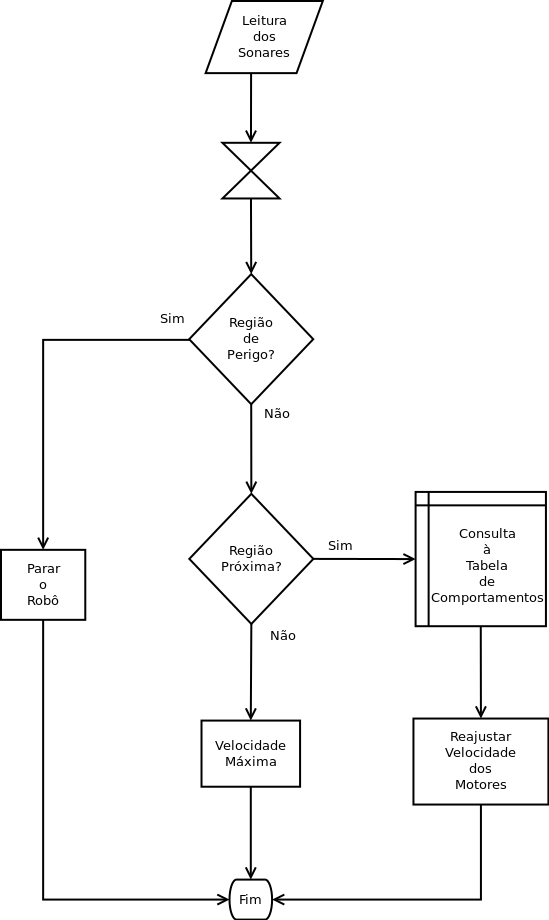
\includegraphics[width=0.8 \linewidth]{../../Imagens/ObstAvoid.png}
    \caption{Fluxograma da Rotina de Desvio de Obstáculos}
    \label{ObstAvoid}
  \end{figure}

\section{Sistemas de Tempo Real}
São sistemas computacionais que dependem não somente que os dados computados estejam corretos, mas que sejam obtidos dentro de um intervalo de tempo 
pré determinado, que pode ser maior ou menor de acordo com a aplicação.
Na literatura, este período em que se espera que a resposta do sistema se dê é denominado \textit{deadline}.
Sistemas de tempo real podem ser classificados em dois tipos: \textit{soft} ou \textit{hard}.

Sistemas \textit{soft} são menos restritivos, tolerando eventuais perdas de \textit{deadline}; 
ao contrário dos sistemas \textit{hard}, em que estas perdas não são aceitáveis.  

Algumas características típicas, apesar de não obrigatórias, de sistemas de tempo real são limitações com relação ao tamanho, propósito específico e 
baixo custo \cite{silberschatz}.

\section{CRC}
Método de detecção de erros aleatórios, isto é, de dados corrompidos ao longo do processo de transmissão ou armazenamento da informação por exemplo 
por ruídos, mas não por um agente \textquoteleft inteligente\textquoteright{} externo que modifique os dados transmitidos, tal qual um 
\textit{malware} \cite{stigge}.

Consiste essencialmente em uma divisão polinomial \cite{stigge}, logo, pode ser implementado em \textit{hardware}, utilizando-se apenas registradores 
de deslocamento com conexões realimentadas \cite{peterson}, assim como em \textit{software}. 
Em suma, trata-se de acrescentar à mensagem digital original um sufixo, que tem seu valor definido por operações realizadas em função da mensagem 
binária que intenta-se enviar e de um polinômio gerador.
Para o \textit{transceiver} nRF24L01+, dois polinômios geradores são utilizados: Eq. \ref{CRC_1} quando o dado cíclico adicionado é de 1 
\textit{byte} , e Eq. \ref{CRC_2}, para 2 \textit{bytes} \cite{nRF}.

Para uma descrição completa de como é implementado este método, vide \cite{stigge,peterson}.

\begin{equation}
\label{CRC_1}
G(X) = X^8 + X^2 + X + 1 
\end{equation}

\begin{equation}
\label{CRC_2}
G(X) = X^{16} + X^{12} + X^5 + 1 
\end{equation}

\section{MIFA} %% se der tempo, né?

\section{efeito hall} %% se der tempo, né?

\section{campo girante}

\section{\textit{schmitt trigger}}

\section{PWM}
A modulação por largura de pulso é uma técnica de modulação que consiste em amostrar e codificar o sinal correspondente à mensagem na largura de um 
trem de pulsos de amplitude fixa, i.e. cada amostra da mensagem é convertida em um pulso retangular cuja duração expressa a amplitude do sinal 
modulante.

Um modulador PWM pode ser implementado utilizando-se um circuito comparador não inversor cuja entrada inversora liga-se à saída de um gerador de 
ondas tipo dente de serra (\textit{trailing edge modulation}), dente de serra invertida (\textit{leading edge modulation}  ou triangular 
(\textit{modulation on both edges}), na entrada não inversora, o sinal modulante. 
Desta forma, quando a tensão da mensagem excede a amplitude da onda gerada, observa-se um sinal alto na saída, caso contrário, baixo, conforme 
ilustra a Fig. \ref{pwm_modulation_types}.

  \begin{figure}[!htb] %% TODO fonte: https://en.wikipedia.org/wiki/File:Three_PWM_types.svg
    \centering
    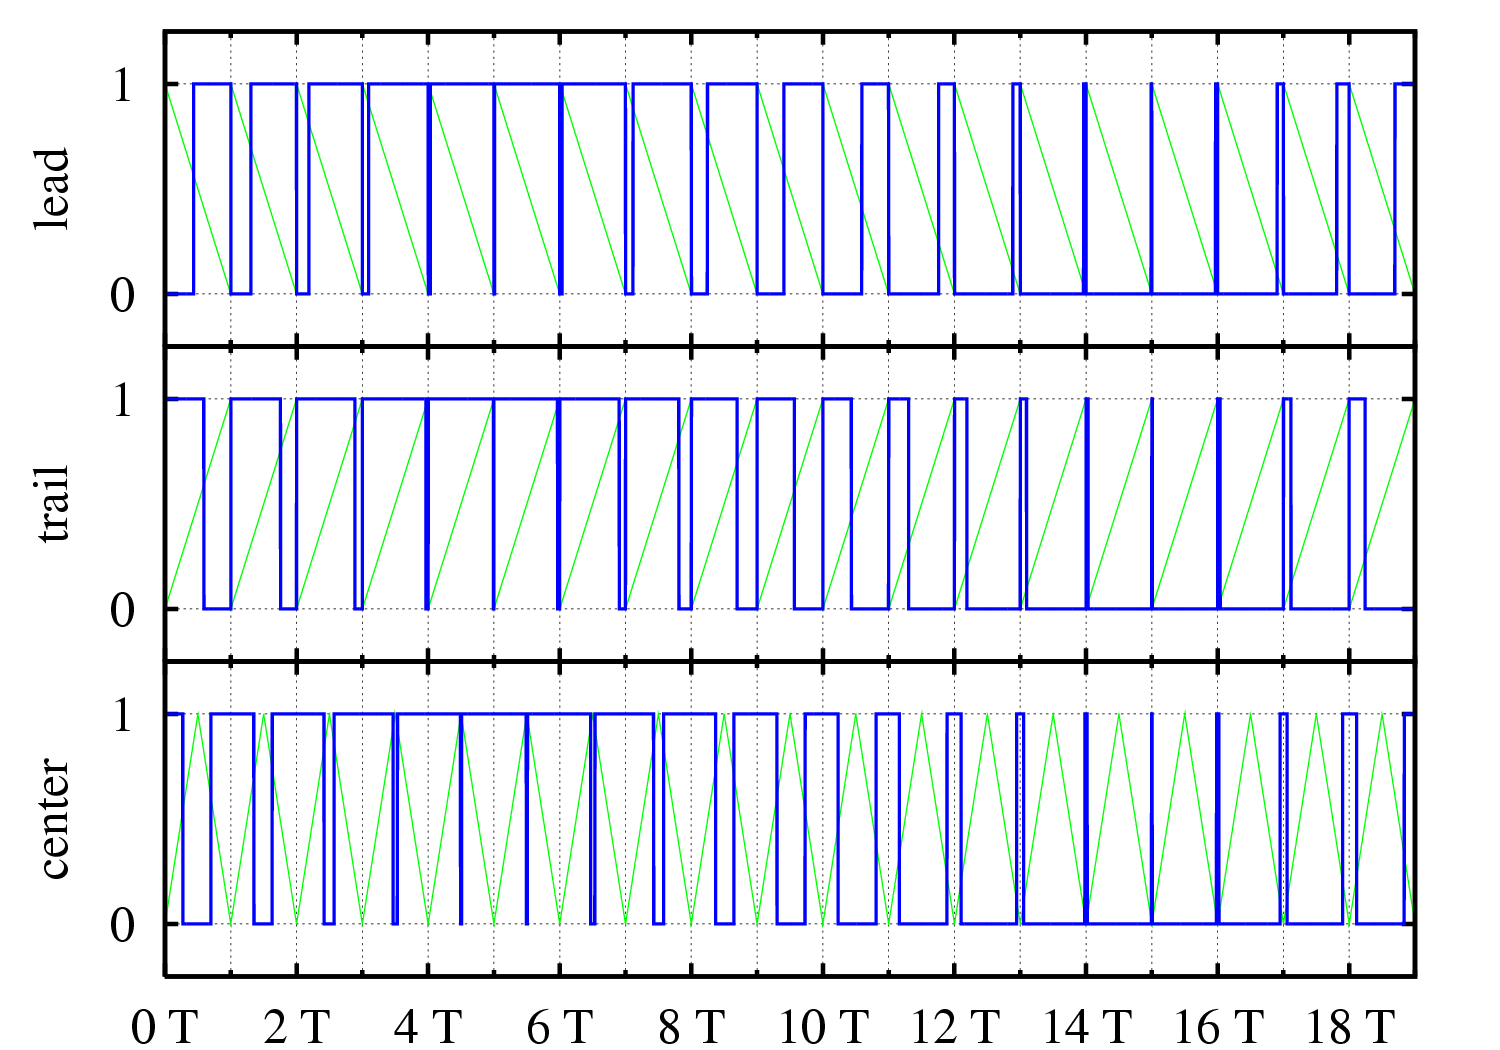
\includegraphics[width=0.7\linewidth]{../../Imagens/PWM_modulation_types.png}
    \caption{Três tipos de modulação PWM: \textit{trailing edge}, \textit{leading edge} e  \textit{both edges}, de cima pra baixo, respectivamente.}
    \label{pwm_modulation_types}
  \end{figure}
  
  %TODO circuito corretor de erros:
   First, the error amplifier accommodates feedback of the output PWM waveform in order to correct for any errors in the
output voltage introduced by the comparator. Second, it adds a dc offset to the input voltage so that negative input voltages can be accommodated by 
the circuit.
 
 Because the supply voltage of the comparator directly impacts the output voltage, PWM circuits without feedback have no power supply rejection. In 
this TI Design, the error amplifier acts as an inverting amplifier to the input signal, shown as a dc-coupled source VIN. By including the comparator 
inside the feedback loop of the error amplifier, and adding integration capacitor C1, the error amplifier now directly controls the average output 
voltage



para uma descrição detalhada do circuito e simulações vide \cite{pwm_modulator}

\section{GFSK}

\section{banda ISM}

\section{SPI}
\end{apendicesenv}
% ---

% ----------------------------------------------------------
% Anexos
% ----------------------------------------------------------

\begin{anexosenv}
% Imprime uma página indicando o início dos anexos
% \partanexos
\chapter{Anexos}
\end{anexosenv}

%---------------------------------------------------------------------
% INDICE REMISSIVO é necessário??
%---------------------------------------------------------------------
%\phantompart
% \printindex
%---------------------------------------------------------------------

\end{document}